\documentclass[aspectratio=169,dvipsnames]{beamer}

%%%% Standard packages
\usepackage[latin1]{inputenc}
\usepackage{graphicx}
\usepackage{amsmath,mathrsfs}
\usepackage{acro}
% Arrows
\usepackage{centernot}
% TikZ & PGF for drawings & flow-charts
\usepackage{pgffor,pgfplots}
\usepackage{tikz}
  \usetikzlibrary{arrows, automata}
  \usetikzlibrary{shapes,arrows}
  \usetikzlibrary{spy}
  \usetikzlibrary{matrix}
  \usetikzlibrary{overlay-beamer-styles}
  \usetikzlibrary{positioning}
  \usetikzlibrary{matrix}
\usepackage{tikz-cd}
 \usepackage{transparent}

%\usetikzlibrary{timeline}
% Handling tables
\usepackage{multirow}
\usepackage{pgfplotstable}
\usepackage{ragged2e}
\usepackage{booktabs,colortbl}
% Packages for typesetting algorithms and good looking pseudocode 
\usepackage{algorithm}
\usepackage[noend]{algpseudocode}
\renewcommand{\thealgorithm}{}
% Handling references
%\usepackage{bibentry}
\usepackage{apacite}
\let\cite\shortcite


%%%% Settings 
%% Settings for hyperref
\hypersetup{%
    bookmarks=true,         % show bookmarks bar?
    pdfmenubar=true,       % show Acrobat's menu?
    pdffitwindow=false,     % window fit to page when opened
    pdfstartview={FitH},    % fits the width of the page to the window
    colorlinks=true,       % false: boxed links; true: colored links
    linkcolor=red,          % color of internal links
    citecolor=gray,        % color of links to bibliography
    filecolor=blue,      % color of file links
    urlcolor=blue,           % color of external links
    pdfborder = {0,0,0}
}
%% Settings for the beamer class.
% Select presentation mode  
\mode<presentation>{%
  \usetheme[height=14mm]{Rochester}
  \setbeamertemplate{items}[ball] 
  \setbeamertemplate{blocks}[rounded][shadow=true]   
  \setbeamertemplate{navigation symbols}{}   
  \setbeamercovered{transparent}%
  \setbeamertemplate{footline}{\hfill \insertframenumber/\inserttotalframenumber \quad}  
}
%  Remove navigation buttons
\beamertemplatenavigationsymbolsempty 
% Place logos in the title page
\titlegraphic{%
  \vskip-3\baselineskip
  
\includegraphics[height=35pt]{SSF_Logotype}
  \hfill
  
\includegraphics[height=35pt]{KTH_Logotype}
}
% Declare image layers
\pgfdeclarelayer{background layer} 
\pgfdeclarelayer{foreground layer}
\pgfsetlayers{background layer,main,foreground layer}
% For every picture that defines or uses external nodes, you'll have to
% apply the 'remember picture' style. to avoid some typing, we'll apply
% the style to all pictures.
\tikzstyle{every picture}+=[remember picture]
% By default all math in TikZ nodes are set in inline mode. Change this to
% displaystyle s\item that we don't get small fractions.
\everymath{\displaystyle}
%% Table 
\setlength{\heavyrulewidth}{0.1em}
\newcommand{\otoprule}{\midrule[\heavyrulewidth]}
%% Location of images, requires 'graphicx' package
\graphicspath{
  {images/}
  {images/LogoTypes/}
  {images/Denoising/}
  {images/SparseLand/}
  {images/InverseProblem/}
  {images/InverseProblem/ImagePossibilities/}
  {images/InverseProblem/Prior/}
  {images/BilevelOpt/}
  {images/BilevelOpt/Denoising/}
}  

%% TikZ
\tikzset{basic/.style={draw,fill=blue!20,text width=1em,text badly centered}}
\tikzset{input/.style={basic,circle}}
\tikzset{weights/.style={basic,rectangle}}
\tikzset{functions/.style={basic,circle,fill=blue!10}}

%%%% Acronyms
\DeclareAcronym{CNN}{
  short = CNN,
  long = convolutional neural network}
\DeclareAcronym{VC}{
  short = VC,
  long = Vapnik-Chervonenkis}
\DeclareAcronym{ReLU}{
  short = ReLU,
  long = rectified linear unit}
\DeclareAcronym{SGD}{
  short = SGD,
  long = stochastic gradient decent}
\DeclareAcronym{CM}{
  short = CM,
  long = conditional mean}
\DeclareAcronym{MAP}{
  short = MAP,
  long = maximum a posteriori}
\DeclareAcronym{DAG}{
  short = DAG,
  long = directed acyclic graph}
  
%%%% Macros
% Sets, spaces, etc
\newcommand{\Real}{\mathbb{R}}
\newcommand{\Natural}{\mathbb{N}}
\newcommand{\Class}[1]{\mathfrak{#1}}
\newcommand{\ModelClass}{\mathscr{M}}
\newcommand{\InputSpace}{X}
\newcommand{\OutputSpace}{Y}
\newcommand{\HSpace}{H}
\newcommand{\HSpaceOther}{H'}
\newcommand{\RecSpace}{X}
\newcommand{\DataSpace}{Y}
\newcommand{\ParamSet}{\triangle}
\newcommand{\Dict}{\mathscr{D}}
\newcommand{\DictMat}{\boldsymbol{\mathsf{D}}}
\newcommand{\GammaMat}{\boldsymbol{\mathsf{\Gamma}}}
\newcommand{\Domain}{\Omega}
\newcommand{\DataDomain}{\mathbb{M}}
\newcommand{\vfield}{\boldsymbol{\nu}}
% Operators
\newcommand{\Op}[1]{\operatorname{\mathcal{#1}}}
\newcommand{\ForwardOp}{\Op{A}}
\newcommand{\ForwardOpMatrix}{\boldsymbol{\mathsf{A}}}
\newcommand{\ForwardOpPseduoInv}{\ForwardOp^{\dagger}}
\newcommand{\LinMap}{\Op{W}}
\newcommand{\NonLinMap}{\Psi}
\newcommand{\Activation}{\psi}
\DeclareMathOperator*{\argmin}{arg\,min}
\DeclareMathOperator{\dist}{d}
\DeclareMathOperator{\Dropout}{Dropout}
\DeclareMathOperator{\Pool}{Pool}
\DeclareMathOperator{\Rad}{Rad}
\DeclareMathOperator{\rank}{rank}
\DeclareMathOperator{\Id}{Id}
\DeclareMathOperator{\LogLikelihood}{\mathcal{L}}
\DeclareMathOperator{\RegFunc}{\mathcal{R}}
\DeclareMathOperator{\prox}{prox}
\DeclareMathOperator{\modulus}{mod}
\DeclareMathOperator{\SynthOp}{S}
\DeclareMathOperator{\Patch}{P}
\DeclareMathOperator{\AnOp}{E}
% Elements
\newcommand{\velem}{x}
\newcommand{\velemother}{y}
\newcommand{\inputvar}{x}
\newcommand{\outputvar}{y}
\newcommand{\signal}{f}
\newcommand{\signaltrue}{\signal^*}
\newcommand{\dataother}{h}
\newcommand{\data}{g}
\newcommand{\datanoise}{\delta\data}
\newcommand{\dataideal}{\data_0}
\newcommand{\param}{\theta}
\newcommand{\valpha}{\boldsymbol{\alpha}}
% Probabilistic notions
\newcommand{\Prob}{\mathbb{P}}
\newcommand{\PClass}[1]{\mathscr{P}_{#1}}
\newcommand{\SAlg}[1]{\mathfrak{S}_{#1}}
\newcommand{\RecSpaceSAlg}{\SAlg{\RecSpace}}
\newcommand{\DataSpaceSAlg}{\SAlg{\DataSpace}}

\DeclareMathOperator{\Expect}{\mathbb{E}}
\DeclareMathOperator{\Risk}{\mathcal{R}}
\newcommand{\model}[1]{\mathcal{A}_{#1}^{\dagger}}
\newcommand{\stochastic}[1]{\mathsf{#1}}
\newcommand{\DataModel}{\mathcal{M}}
\newcommand{\stvelem}{\stochastic{\velem}}
\newcommand{\stvelemother}{\stochastic{\velemother}}
\newcommand{\stsignal}{\stochastic{\signal}}
\newcommand{\stdata}{\stochastic{\data}}
\newcommand{\stparam}{\stochastic{\param}}
\newcommand{\stinputvar}{\stochastic{\inputvar}}
\newcommand{\stoutputvar}{\stochastic{\outputvar}}
\newcommand{\stsigma}{\stochastic{\sigma}}
\newcommand{\ProbSignalTrue}{\mu^*}
\newcommand{\prior}{\pi_{\text{prior}}}
\newcommand{\likelihood}[2]{\pi_{\text{liklh}}\left(#1 \left\mid\right. #2\right)}
\newcommand{\posterior}[2]{\pi_{\text{post}}\left(#1 \left\mid\right. #2\right)}
% NN notions
\newcommand{\Learn}{\mathcal{L}}
\newcommand{\NNMatrix}{\boldsymbol{W}}
\newcommand{\tData}{\Sigma}
\newcommand{\optimParam}{\param^*}
\newcommand{\optimParamEmp}{\widehat{\param}^*}
\DeclareMathOperator{\pregfunc}{\mathcal{S}}
\DeclareMathOperator{\loss}{\ell}
\newcommand{\depth}{d}
\newcommand{\layerdim}{n}
\newcommand{\paramdim}{N}
\newcommand{\trainData}{\Sigma_{\text{train}}}
\newcommand{\trainDatadim}{m}
\newcommand{\trainProbMeas}{\widehat{\mu}_{\text{train}}}
\newcommand{\trainError}{\epsilon_{\text{train}}}
\newcommand{\testData}{\Sigma_{\text{test}}}
\newcommand{\testDatadim}{{m'}}
\newcommand{\testProbMeas}{\widehat{\mu}_{\text{test}}}
\newcommand{\testError}{\epsilon_{\text{test}}}
\newcommand{\genError}{\epsilon_{\text{gen}}}
% Other
\newcommand{\captionfix}[1]{\vbox to 20pt {\vfil \hbox to \columnwidth{\hfill #1 \hfill} \vfil}}
\makeatletter
\def\parsecomma#1,#2\endparsecomma{\def\page@x{#1}\def\page@y{#2}}
\tikzdeclarecoordinatesystem{page}{
    \parsecomma#1\endparsecomma
    \pgfpointanchor{current page}{north east}
    % Save the upper right corner
    \pgf@xc=\pgf@x%
    \pgf@yc=\pgf@y%
    % save the lower left corner
    \pgfpointanchor{current page}{south west}
    \pgf@xb=\pgf@x%
    \pgf@yb=\pgf@y%
    % Transform to the correct placement
    \pgfmathparse{(\pgf@xc-\pgf@xb)/2.*\page@x+(\pgf@xc+\pgf@xb)/2.}
    \expandafter\pgf@x\expandafter=\pgfmathresult pt
    \pgfmathparse{(\pgf@yc-\pgf@yb)/2.*\page@y+(\pgf@yc+\pgf@yb)/2.}
    \expandafter\pgf@y\expandafter=\pgfmathresult pt
}
\makeatother
\newcommand{\advantage}{\textcolor{PineGreen}{$\boldsymbol{+}$}}
\newcommand{\drawback}{\textcolor{WildStrawberry}{$\boldsymbol{-}$}}
\newcommand{\deAlert}[1]{{\color{gray}\transparent{0.01} #1}}
\newcommand{\slideTitle}[1]{\begin{center}{\Huge \structure{#1}}\end{center}}
\newcommand{\Cdot}{\,\cdot\,}


% Preamble 
\title{Lecture 2: Machine learning in the context of inverse problems - Learning priors and post-processing}
\author{Ozan �ktem \and Jonas Adler}
\institute{Department of Mathematics \\ KTH - Royal Institute of Technology, Stockholm}
\date{April 18, 2018 \\ 
Mini-course: Mathematics of Deep Learning \\ with an Emphasis on Inverse Problems \\[0.5em]
Georg-August-Universit�t G�ttingen}

\begin{document}
\maketitle

% Frame
\begin{frame}{Lecture overview}
\begin{itemize}
\item Inverse problems and regularisation
  \begin{itemize}
  \item Ill-posedness \& regularisation
  \item Analytic methods
  \item Iterative methods with early stopping
  \item Variational methods
  \end{itemize}
\item Learning parameters in regulariser
  \begin{itemize}
  \item Bi-level optimisation
  \item Examples of bi-level optimisation
  \end{itemize}
\item Sparse models
  \begin{itemize}
  \item  Sparse recovery
  \item Joint reconstruction \& dictionary learning
  \item Dictionary learning
  \item Convolutional Sparse Model
  \end{itemize}
\item Prior with black box denoiser  
\end{itemize}
\end{frame}


% Frame
\begin{frame}[plain]
\slideTitle{Inverse problems and regularisation}
\end{frame}

\begin{frame}{Inverse problem}
% Inverse problem
\structure{Inverse problem:} 
  Recover (reconstruct) an estimate of signal $\signaltrue \in \RecSpace$ from data $\data \in \DataSpace$ assuming 
  \begin{equation*}
    \data = \ForwardOp(\signaltrue) + \datanoise.  
  \end{equation*}    
  \begin{itemize}
  \item \structure{Reconstruction space:} $\RecSpace$ (normed) vector space, elements represent possible signals.
    We consider $\RecSpace \subset$ real valued functions defined on $\Domain \subset \Real^n$.
  \item \structure{Data space:} $\DataSpace$ (normed) vector space, elements represent possible data.
      We consider $\DataSpace \subset$ real valued functions defined on manifold $\DataDomain$.
      \par \structure{Acquisition geometry:} Digitisation of data, i.e., sampling scheme in $\DataDomain$.
  \item \structure{Forward operator:} $\ForwardOp \colon \RecSpace \to \DataSpace$, the deterministic part of a simulator (mathematical model) for how data is generated.
  \item \structure{Data noise component:} $\datanoise$ generated by a $\DataSpace$-valued random variable.
  \item \structure{Data noise level:} $\delta := \Vert \datanoise \Vert_{\DataSpace}$.
  \item \structure{Reconstruction (operator):} Mapping $\ForwardOp^{\dagger} \colon \DataSpace \to \RecSpace$ such that $\ForwardOp^{\dagger}(\data) \approx \signaltrue$.
  \end{itemize}
\end{frame}

% Frame
\begin{frame}{Ill-posedness}% Ill-posedness
\begin{columns}[T]
\begin{column}{0.45\textwidth} 
  \begin{itemize}
  \item \structure{Inverse problem:} Recover $\signaltrue \in \RecSpace$ from $\data = \ForwardOp(\signaltrue) + \datanoise$.
  \item \structure{Ill-posedness}
    \begin{itemize}
      \item \alt<1-2>{\alert<1-2>{Existence}}{\deAlert{Existence}}
      \visible<3->{
        \item \alert<3>{Uniqueness} 
        \item \alert<3>{Stability}
      }
      \end{itemize}
  \visible<5->{\item \structure{Well-defined regularisation:} Existence and stability.}      
  \end{itemize}
\end{column}
\begin{column}{0.6\textwidth}
  \begin{overprint}
  \onslide<2-3>
    \begin{itemize}
    \item \structure{Existence:} Relax notion of a solution, e.g., 
       \[ \min_{\signal \in \RecSpace} \LogLikelihood\bigl(\ForwardOp(\signal),\data\bigr) \]
       given $\LogLikelihood \colon \DataSpace \times \DataSpace \to \Real$ (data discrepancy).
    \visible<3>{\item \structure{New difficulties:}
      \begin{itemize}
      \item Multiple (possibly infinitely many) solutions.
      \item Generic solution not continuous w.r.t. data.
      \end{itemize}}
    \end{itemize}
    \onslide<4->    
    \begin{itemize}
    \item \structure{Regularisation:} Replace original ill-posed inverse problem by a well-posed one 
      that is convergent as noise level tends to zero. 
    \item \structure{Key components:}
      \begin{itemize}
      \item \structure{Data model:} Forward operator $\ForwardOp$ and \alert<6-9>{statistical properties of data}.
      \item \structure{Prior model:} A priori info. about $\signaltrue$.
      \item \structure{Regularisation parameter:} Compromise between fitting data and stability, usually based on an estimate of the noise level.
      \end{itemize}
  \end{itemize}
\end{overprint}  
\end{column}
\end{columns}
\par\bigskip
\alt<6-8>{%
  \structure{Statistical properties of data:} 
    Captured by data discrepancy $\LogLikelihood \colon \DataSpace \times \DataSpace \to \Real$, a suitable affine transform 
    of negative log-likelihood of data \cite{Bertero:2008aa}.
}
{\visible<9>{\structure{Main challenges:}}}
%\alt<6-9>{\structure{Statistical Properties of data:} \visible<7-9>{Data discrepancy $\LogLikelihood \colon \DataSpace \times \DataSpace \to \Real$.}}{\visible<10>{\structure{Main challenges:}}}
\begin{overprint}
%\onslide<6>
%\begin{itemize}
%\item
%Captured by data discrepancy $\LogLikelihood \colon \DataSpace \times \DataSpace \to \Real$ that is given as a suitable affine transform 
%of negative log-likelihood of data \cite{Bertero:2008aa}.
%\end{itemize}
\onslide<6>
\begin{itemize}
\item
Additive Gaussian noise (zero mean, covariance $\Sigma$):
$\LogLikelihood(\data, \dataother) :=\Vert \data-\dataother \Vert^2_{2}$ or 
$\LogLikelihood(\data, \dataother\bigr) := 
               \Vert \data-\dataother \Vert_{\Sigma^{-1}}^2$.               
\end{itemize}
\onslide<7>
\begin{itemize}
\item
Poisson data (mean = measurement):
$\LogLikelihood(\data,\dataother) := 
                   \sum_{i=1}^m  \bigl[ \dataother_i \log \data_i - \data_i \bigr]$.
\end{itemize}
\onslide<8>
\begin{itemize}
\item
Impulse noise, e.g., salt and pepper noise:
$\LogLikelihood( \data, \dataother ) := \Vert \data-\dataother \Vert_{0}$
or
$\LogLikelihood( \data, \dataother ) := \Vert \data-\dataother \Vert_{1}$.      
\end{itemize}
\onslide<9>
\begin{itemize}
\item Choosing prior model $\implies$ reconstruction is a well-defined regularisation.
\item Choose regularisation parameter.
\item Computationally feasible data model.
\end{itemize}
\end{overprint}     
\end{frame}

\begin{frame}{Regularisation theory}{Type of mathematical results}
\begin{itemize}
\item \structure{Inverse problem:} Recover $\signaltrue \in \RecSpace$ from $\data = \ForwardOp(\signaltrue) + \datanoise$.
\item \structure{Reconstruction method:} Parametrised family $\{ \model{\param} \}_{\param}$ where 
  $\model{\param} \colon \DataSpace \to \RecSpace$.
\item \structure{Existence:}
   For every $\data \in \DataSpace$, there exist a solution $\model{\param}(\data) \in \RecSpace$ given fixed $\param$.
   \par $\implies$ Makes it possible to define reconstruction method as mapping.
\item \structure{Stability:}
   $\data \mapsto \model{\param}(\data)$ is continuous in relevant topology for fixed $\param$.
   \par $\implies$ Small variations in data does not result in large variations in reconstruction. 
\visible<2->{   
\item \structure{Convergence:}
  $\signal_{\param,\delta} := \model{\param}(\dataideal + \datanoise)$ where $\dataideal := \ForwardOp(\signaltrue)$ and  
  $\delta := \Vert \datanoise \Vert$. Show that there exists decreasing $\delta \mapsto \param(\delta)$ (parameter selection rule) such that 
  \[ \signal_{\param(\delta),\delta} \to \signal 
     \quad\text{as $\delta \to 0$ where $\signal$ solves $\ForwardOp(\signal)=\dataideal$.}
  \]   
}
\visible<3->{
\item\vskip-\baselineskip     
 \structure{Convergence rates:}
  Estimate difference between $\signal_{\param,\delta}$ and a minimal norm solution.
  Need regularity assumptions of $\signaltrue$ (source conditions).
\item \structure{Stability estimates:}
 Bounds to the difference between $\signal_{\param,\delta}$ and $\signal_{\param,0}$ depending on $\delta$.
 }
\end{itemize}
\end{frame}

\begin{frame}{Inverse problems}{Denoising}
\begin{itemize}
\item \visible<1->{
Inverse problem: $\ForwardOp=\Id \implies$ remove noise from a signal/image.
}
\item \visible<4->{
Removal of additive zero-mean white noise is essentially a solved problem in image processing
}
\end{itemize}
\begin{columns}
\begin{column}{0.27\textwidth}
  \centering
  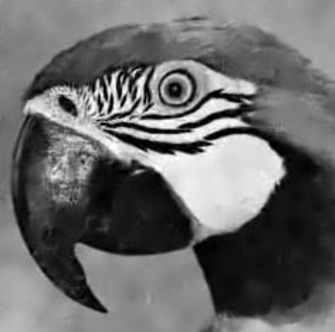
\includegraphics[width=\textwidth]{original_image}
  \par
  Signal: Original image
\end{column}
\hfill \visible<2->{{\Huge $+$}} \hfill
\begin{column}{0.27\textwidth}
  \centering
  \visible<2->{
  
\includegraphics[width=\textwidth]{WhiteNoise}
  \par
  Noise}
\end{column}
\hfill \visible<3->{{\Huge $=$}} \hfill
\begin{column}{0.27\textwidth}
  \centering
  \visible<3->{
  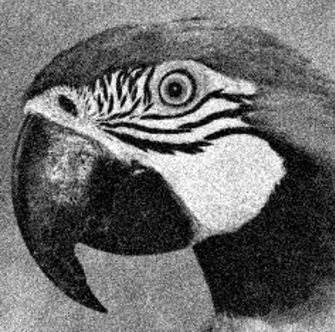
\includegraphics[width=\textwidth]{noisy_image}
  \par
  Data: Noisy image}
\end{column}
\end{columns}
\end{frame}


\begin{frame}{Inverse problems}{Other}
\begin{itemize}
\item Deconvolution: $\ForwardOp(\signal) = k \ast \signal$ 
  \begin{itemize}
  \item $k$ kernel.
  \item $k$ unknown (blind deconvolution).
  \end{itemize}
\item Tomography: $\ForwardOp(\signal)(\ell) = \int_{\ell} \signal$.
\item PDE parameter estimation: Forward operator = solution to a PDE.
\item \ldots
\end{itemize}
\end{frame}


\begin{frame}{Type of regularisation methods}
\begin{itemize}
\item Analytic methods. %
\item Iterative methods with early stopping.
\item Variational methods.
\item \deAlert{Learned iterative methods.}
\end{itemize}
\end{frame}

\begin{frame}{Analytic methods}
\begin{itemize}
\item \structure{Data model:} 
  $\data=\ForwardOp(\signaltrue)$, i.e., no specific adaptation to handle noise.
\item \structure{Prior model:} Features of $\signaltrue$ stably recoverable, e.g., if feature is a mollified version $\implies$ signal is bandlimited.
\item \structure{Reconstruction method:}
  Highly specific (depends on forward operator and acquisition geometry).
  $\model{\param}(\data) =$ stably recoverable features of $\signaltrue$, main example is when features is a mollified version of the signal.
\item \structure{Regularisation parameter:}  
  $\param$ parametrises features, e.g., if feature is a mollified version then $\param$ is typically the bandlimit, which is 
  set using Shannon-Nyquist sampling theory.
\item Examples:
  \begin{itemize}
  \item Filtered backprojection: Recovering bandlimited function from its ray transform data \cite{Natterer:2001aa}. 
  \item Lambda-tomography: Recovering wavefront set (singularities) of function from its ray transform data \cite{Quinto:1993aa,Krishnan:2015aa}.
  \item Approximate inverse \cite{Sc07,Louis:1996aa}.
\end{itemize}
\end{itemize}
\end{frame}

\begin{frame}{Iterative regularisation with early stopping}
\begin{itemize}
\item \structure{Data model:} 
  Both forward operator and data discrepancy $\LogLikelihood \colon \DataSpace \times \DataSpace \to \Real$ are exchangeable.
\item \structure{Prior model:} Iterates are semi-convergent. 
\item \structure{Reconstruction method:}
  $\model{\param}(\data)$ given by a fixed point iteration scheme for minimising $\signal \mapsto \LogLikelihood\bigl( \ForwardOp(\signal), \data \bigr)$.
\item \structure{Regularisation parameter:} $\param$ number of iterates.
\item Examples:
  \begin{itemize}
  \item Conjugate gradient least squares with variants \cite{EnHaNe00,Bakushinsky:2004aa,KaNeSc08,Burger:2015aa}.
  \item Algebraic reconstruction technique with variants \cite{Hansen:1997aa,Byrne:2008aa}.
  \item ML-EM \cite{Natterer:2001aa,Byrne:2015aa}.
\end{itemize}
\end{itemize}
\end{frame}

\begin{frame}{Variational regularisation}
\begin{itemize}
\item \structure{Data model:} 
  Both forward operator and data discrepancy $\LogLikelihood \colon \DataSpace \times \DataSpace \to \Real$ are exchangeable.
\item \structure{Prior model:} 
  Accounted for by regulariser $\RegFunc_{\param} \colon \RecSpace \to \Real$. 
\item \structure{Reconstruction method:}
  $\model{\param}(\data)$ is solution to a variational problem (penalised log-likelihood):
  \begin{equation*}
    \min_{\signal \in \RecSpace} \bigl[ \LogLikelihood\bigl(\ForwardOp(\signal), \data\bigr) + \RegFunc_{\param}(\signal) \bigr]
  \quad\text{for a fixed $\param$.} 
  \end{equation*}
\item \structure{Regularisation parameter:} $\param$ parametrises regulariser.
\item Examples:
  \begin{itemize}
  \item Tikhonov regularisation \cite{EnHaNe00}.
  \item Total variation regularisation \cite{ScGrGrHaLe09,Caselles:2015aa}.
  \item \ldots
\end{itemize}
\end{itemize}
\end{frame}


\begin{frame}{Variational regularisation methods}{Common prior models} 
{\scriptsize 
     \begin{center}
     \begin{tabular}{>{\RaggedRight} p{0.4\textwidth} >{\RaggedRight} p{0.55\textwidth}}
        \multicolumn{1}{ c }{\textbf{Prior information}}  
       &  \multicolumn{1}{ c }{\textbf{Regularisation functional} $\RegFunc_{\param}(\signal) := \param \RegFunc(\signal)$} \\
     \otoprule  
     \multirow{1}{0.5\textwidth}{$\signaltrue - \rho$ is sparse for some known $\rho \in\RecSpace$.}
       & $\RegFunc(\signal) = \Vert \signal - \rho \Vert_{p}$ with $0\leq p \leq 1$ \\
%       = 
%             \left( \int_{\Domain} \bigl\Vert \signal(x) - \rho(x) \bigr\vert^p \,dx\right)^{1/p}$ with $0\leq p \leq 1$   \\
       & \\
       & $\RegFunc(\signal) =\int_{\Domain} \Bigl( \signal(x) \ln\frac{\signal(x)}{\rho(x)}-\signal(x)+\rho(x) \Bigr)dx$  \\      
     \midrule  
       $\nabla \signaltrue$ is sparse.
       
       & $\RegFunc(\signal) = \Vert \nabla f \Vert_{p} = 
             \left( \int_{\Domain} \bigl\vert \nabla \signal(x) \bigr\vert^p \,dx \right)^{1/p}$
           with $0\leq p \leq 1$. \\             
      & Case with $p=1$ is TV-regularisation.\\
%     \midrule          
%        $\signaltrue$ is a cartoon function, i.e., smoothly varying inside regions in $\Domain$.
%%        Adapt the gradient exponent to fit the data, so that near edges it behaves exactly 
%%        like TV-regularsiation and away from the edges it may behave more like the 
%%        Dirichlet energy. 
%        & $\RegFunc(\signal) =  \int_{\Domain} \bigl\vert \nabla \signal(x) \bigr\vert^{p(\vert \nabla \signal(x) \vert)} \,dx$
%           $p \colon \Real_+ \to [1,2]$ is monotonically decreasing. 
%           \par \quad \par
%           $\RegFunc(\signal) = \min_{\nu} \bigl[ \Vert \nabla \signal - \nu \Vert_1 + \theta \Vert \nabla \nu \Vert_1 \bigr]$ 
%           where $\nabla \nu$ is the symmetrised gradient of the vector-field $\nu$.
%         \\
%     \midrule
%       Edges in $\signaltrue$ are better characterised along specific directions that are a priori known.
%%       Emphasise certain edge directions so that they are preferred in reconstructions,
%%       \eg when one seeks to restore characteristic functions of convex regions having desired 
%%       shapes.
%       & $\RegFunc(\signal) =  \int_{\Domain} \phi\bigl( \vert \nabla \signal(x) \vert \bigr) \,dx$
%          where $\phi \colon \Real^n \to \Real$ is convex, zero at the origin, and positively 1-homogenous. \\     
     \midrule     
       $\signaltrue$ is smooth.
%       Minimise the Dirichlet energy       
       & $\RegFunc(\signal) = \Vert \nabla f \Vert_{2} = 
               \sqrt{\int_{\Domain} \bigl\vert \nabla \signal(x) \bigr\vert^2 \,dx}$. \\
     \midrule
       $\signaltrue$ is sparse w.r.t. $\{ \phi_i \}_i$.
       & $\RegFunc(\signal) = \Bigl( \sum_i \vert \langle \signal, \phi_i \rangle  \vert^p \Bigr)^{1/p}$ with $0\leq p \leq 1$. \\
     \bottomrule
     \end{tabular} 
     \end{center}  
}
\end{frame}

%\begin{frame}{Variational regularisation methods}{Common parameter choice rules}
%   Choice based on specific form of data discrepancy $\LogLikelihood \colon \DataSpace \times \DataSpace \to \Real$.
%   $\signal_{\param} := \model{\param}(\data)$ denotes regularised solution. 
%  {\scriptsize 
%     \begin{center}
%     \begin{tabular}{>{\RaggedRight} p{0.4\textwidth} >{\RaggedRight} p{0.5\textwidth}}
%            \multicolumn{1}{ c }{\textbf{Prior knowledge}}  
%       &  \multicolumn{1}{ c }{\textbf{Principle}} \\
%     \otoprule  
%       \multirow{1}{0.4\textwidth}{A posteriori rules: Access to estimate of the data error and/or the value of 
%       the regularisation functional: 
%       Know $\epsilon>0$ such that $\LogLikelihood\bigl( \ForwardOp(\signaltrue), \data \bigr) < \epsilon$ and/or
%       $\delta>0$ such that $\RegFunc(\signaltrue)\leq \delta$.
%       }
%       & Morozov principle: Choose $\param$ so 
%         $\LogLikelihood\bigl( \ForwardOp(\signal_{\param}), \data \bigr) \leq \epsilon$. 
%         \par\quad\par 
%         Miller method: Choose $\param$ so 
%         $\LogLikelihood\bigl( \ForwardOp(\signal_{\param}), \data \bigr) < \epsilon$ and 
%         $\RegFunc(\signal_{\param})\leq \delta$. \\
%       & \\
%     \midrule       
%       \multirow{1}{0.4\textwidth}{A priori rules: No a priori knowledge about the data error and/or the 
%          value of the regularisation functional. Let the data $\data$ choose the value of regularisation
%          parameter.}
%       & Generalised cross-validation: Let $\signal_{k,\param}\in\RecSpace$ denote the regularised solution 
%           when we have removed  the $k$:th component $\data_k$ of the data $\data$.  
%           Choose $\param$ in order to predict missing data values, i.e., 
%          $\ForwardOp(\signal_{k,\param})_k \approx \data_k$ by minimising
%          $\sum_{i=1}^m \bigl\vert \ForwardOp(\signal_{k,\param}) - \data_k \bigr\vert$.          
%         \par\quad\par 
%          L-curve: $\param$ is chosen where log-log plot of  
%          $\param \mapsto \Bigl( \LogLikelihood\bigl( \ForwardOp(\signal_{\param}),\data \bigr),  \RegFunc(\signal_{\param}) \Bigr)$ 
%          has highest curvature (i.e., a corner). \\       
%     \bottomrule
%     \end{tabular} 
%     \end{center}  
%     }
%\end{frame}

\begin{frame}{Variational regularisation methods}{Common parameter choice rules}
\structure{Three type of methods:}
  A posteriori, a priori, and error-free parameter choice rules \cite{EnHaNe00} \cite[Section~5.6]{Bertero:1998aa}.
\begin{overprint}
\onslide<1>
\structure{A posteriori rules:}
Access to a reasonably tight estimate of the data discrepancy and/or value of regulariser at true solution, i.e., know $\epsilon>0$ and/or $E>0$ such that 
\[
  \LogLikelihood\bigl( \ForwardOp(\signaltrue), \data \bigr) \leq \epsilon
  \quad\text{for $\data := \ForwardOp(\signaltrue) + \datanoise$}
  \qquad\text{and/or}\quad
  \RegFunc(\signaltrue)\leq E.
\]
\vskip-0.5\baselineskip
\begin{itemize}
\item Morozov principle: Choose $\param$ so $\LogLikelihood\bigl( \ForwardOp(\signal_{\param}), \data \bigr) \leq \epsilon$
   \cite{Morozov:1966aa}.
\item Miller method: Choose $\param$ so that 
  $\LogLikelihood\bigl( \ForwardOp(\signal_{\param}), \data^{\delta} \bigr) \leq \epsilon$
  and
  $\RegFunc(\signal_{\param})\leq E$ \cite{Miller:1970aa}.
\end{itemize}
Here, $\signaltrue$ is the true (unknown) solution and $\signal_{\param} := \model{\param}(\data)$ is the regularised solution.
\onslide<2>
\structure{A priori rules:}
Determine the regularisation parameter solely from knowledge of the noise level in data. 
\onslide<3>
\structure{Error-free parameter choice rules:}
Use data to guide choice of parameter, e.g., by balancing principles between the error in the fidelity and the regularisation terms.
\begin{itemize}
\item Generalised cross-validation: Let $\signal_{k,\param}\in\RecSpace$ denote the regularised solution 
  when we have removed  the $k$:th component $\data_k$ of the data $\data$.  
  Choose $\param$ in order to predict missing data values \cite{Golub:1979aa}, i.e., 
  \vskip-0.75\baselineskip  
  \[ \ForwardOp(\signal_{k,\param})_k \approx \data_k
     \quad\text{by minimising}\quad
    \sum_{i=1}^m \bigl\vert \ForwardOp(\signal_{k,\param}) - \data_k \bigr\vert.
  \]    
\item  \vskip-0.25\baselineskip  
 L-curve: $\param$ is chosen where log-log plot of  
  $\param \mapsto \bigl( \LogLikelihood\bigl( \ForwardOp(\signal_{\param}),\data \bigr),  \RegFunc(\signal_{\param}) \bigr)$ 
  has highest curvature (i.e., a corner) \cite{Hansen:1992aa}. 
\end{itemize}
\onslide<4>
\structure{Current status:}
\begin{itemize}
\item Most of the work on parameter choice techniques addresses the case of a single scalar parameter.
\item Much of the theory is developed for additive Gaussian noise, i.e., when data discrepancy $\LogLikelihood$ is a $2$-norm.
\item For error-free parameter choice rules, convergence $\signal_{\param(\delta)} \to \signaltrue$ as $\delta \to 0$ cannot be guaranteed \cite{Bakushinskii:1984aa}.
\item Error-free parameter choice rules computationally very demanding (requires solutions for varying values of regularisation parameter).
\item Although many rules have been proposed, very few of them are used in practice.
\end{itemize}
\end{overprint}
\end{frame}


% Frame
\begin{frame}[plain]
\slideTitle{Learning parameters in regulariser}
\end{frame}


% Frame
\begin{frame}{Bi-level optimisation}
\structure{Variational model:} Define $\model{\param} \colon \DataSpace \to \RecSpace$ as 
\[ \model{\param}(\data) \in \argmin_{\signal} \Bigl[ \LogLikelihood\bigl( \ForwardOp(\signal),\data \bigr) + \RegFunc_{\param}(\signal) \Bigr]
    \quad\text{for $\data \in \DataSpace$.} 
\]
\begin{itemize}
\item Supervised training data $(\signal_i,\data_i) \in \RecSpace \times \DataSpace$ such that $\data_i \approx \ForwardOp(\signal_i)$.
\item Learn regularisation parameter $\param$ from supervised training data by minimising empirical risk:
\[
   \param^* \in \argmin_{\param} \Bigl[ \frac{1}{m} \sum_{i=1}^m \loss_{\RecSpace}\bigl(\model{\param}(\data_i),\signal_i\bigr) \Bigr]
\]
where $\loss_{\RecSpace} \colon \RecSpace \times \RecSpace \to \Real$ is a loss function.
\end{itemize}
\end{frame}

\begin{frame}{Bi-level optimisation}
\begin{itemize}
\item \structure{Bi-level optimisation:} Find reconstruction method $\model{\param^*} \colon \DataSpace \to \RecSpace$ from training data $(\signal_i,\data_i)$ where
\[
\begin{cases}
   \param^* \in \argmin_{\param} \Bigl[ \frac{1}{m} \sum_{i=1}^m \loss_{\RecSpace}\bigl(\model{\param}(\data_i),\signal_i\bigr) \Bigr] 
   & \\[1.5em]
   \model{\param}(\data) \in \argmin_{\signal} \Bigl[ \LogLikelihood\bigl( \ForwardOp(\signal),\data \bigr) + \RegFunc_{\param}(\signal) \Bigr] &
\end{cases}
\]
\item $\param^*$ yields a minimiser of the variational model that minimises the empirical risk.
\item Existence of solution to bi-level optimisation far from obvious, needs to be proved. 
  Uniqueness does not hold in general. 
\item Computing derivative of $\param \mapsto \model{\param}(\data)$ is non-trivial and computationally demanding. 
\end{itemize}
\end{frame}


\begin{frame}{Example of bi-level optimisation}
\begin{overprint}
\onslide<1-2> % Slides 1-2
\structure{Anisotropic weighted Dirichlet/total variation:} \cite{Haber:2003aa}
\begin{align*}
  \RegFunc_{\param}(\signal) := \bigl\Vert \param(\Cdot) \nabla \signal(\Cdot) \bigr\Vert^2_2 &\quad \text{where $\param \colon \Domain \to \Real$} 
  \\[0.5em]
  \RegFunc_{\param}(\signal) := \Bigl\Vert \param\bigl(\vert \nabla \signal(\Cdot) \vert \bigr) \Bigr\Vert_1 &\quad \text{where $\param \colon \Real \to \Real$} 
\end{align*}
\visible<2>{
\structure{Total generalised variation:} 2nd order case (TGV${}^2$) \cite{Bredies:2010aa}:
  \vskip-0.5\baselineskip
  \[ \RegFunc_{\param}(\signal) = \min_{\vfield} \Bigl[ \theta_1 \Vert \nabla \signal - \vfield \Vert_1 + \theta_2 \Vert \boldsymbol{\nabla} \vfield \Vert_1 \Bigr]
     \quad\text{where $\vfield \colon \Real^n \to \Real^n$}
  \]
  \vskip-0.5\baselineskip
  with $\param = (\theta_1,\theta_2) \in \Real^2$ and $\boldsymbol{\nabla} \vfield := \Bigl[ \frac{1}{2}(\partial_j \nu_i + \partial_i \nu_j) \Bigr]_{i,j}$ (symmetrised gradient).
  \begin{itemize}
  \item Denoising using Huber-smoothed version of TGV${}^2$ with an added $H^1$-regularisation incl. proof of existence and algorithms  
    \cite{De-los-Reyes:2017aa}.
  \item Denoising using Infimal Convolution Total Variation \cite{De-los-Reyes:2017aa}.
  \end{itemize}
}  
\onslide<3> % Slide 3
\structure{Weighted sum of $\ell^p$-regularisers:}
Given linear $K \colon \RecSpace \to \RecSpace$,
\[ \RegFunc_{\param}(\signal) := \frac{1}{p} \sum_{i=1}^N \param_i \bigr\Vert K(\signal) \bigl\Vert_p^p 
   \quad\text{with $\param = (\param_i)_i \in \Real^N$.}
\]   
\begin{itemize}
\item $p=1$ generalises total variation.
\item Denoising incl. proof of existence for $p=1,2$ \cite{Kunisch:2013aa}.
\item Semi-smooth Newton algorithm can be used to solve the bilevel optimisation problem for $p=1,2$ \cite{Kunisch:2013aa}.    
\end{itemize}
\onslide<4>  % Slide 4
\structure{Field of Experts model:} Given $\rho \colon \Real \to \Real$ (potential function), 
\[ \RegFunc_{\param}(\signal) := \sum_{i=1}^N w_i \biggl[ \int_{\Domain} \rho\bigl( (\signal \ast k_i)(x) \bigr) dx \biggr] 
   \quad\text{with $\param = (w_i,k_i)_i \in (\Real \times \RecSpace)^N$.}
\]
\begin{itemize}
\item Filters $k_i \colon \Domain \to \Real$ parametrised by finite dimensional parameters:
  \begin{itemize}
  \item Standard finite difference approximations of first- and second-order derivatives 
  \item Higher-order linear operators obtained from dictionary atoms, like basis vectors of the discrete cosine transform \cite{Kunisch:2013aa}.
  \end{itemize}
\item Denoising \cite{Samuel:2009aa,Kunisch:2013aa}.
\item Possible to learn regularisation terms and parameters from the training data using a deep neural network, leads to the `Learned Experts' Assessment-based Reconstruction Network (LEARN)' method \cite{Chen:2018aa}.
\end{itemize}
\onslide<5-6> % Slides 5-6
\structure{Nonconvex fields of experts model:}
\[ \RegFunc_{\param}(\signal) := \sum_{i=1}^N w_i \biggl[ \int_{\Domain} \rho_i\bigl( (\signal \ast k_i)(x) \bigr) dx \biggr]
   \quad\text{with $\param = (w_i,\rho_i,k_i)$.}
\]   
\alt<5>%
{
\vskip-0.5\baselineskip
\begin{itemize}
\item Filters $k_i \colon \Domain \to \Real$ and potential functions $\rho_i \colon \Real \to \Real$ parametrised 
  by finite dimensional parameters.
\item Denoising \cite{Roth:2009aa,Chen:2014aa}.
\item Computing gradients of empirical risk w.r.t. $\param$ can be done via implicit differentiation, very time consuming \ldots
\item 2D denoising example \cite{Chen:2014aa}: $N=80$, filters $k_i \colon \Real^2 \to \Real$ symmetric with $9 \times 9$ pixel support, and  
  $\rho_i(t) = \lambda_i \log(1+ \beta_i t^2) \implies \param \in \Real^{6480}$.
  \par\smallskip Training on test data with $m=200$ images took two weeks!
\end{itemize}
}
{
\begin{columns}
\begin{column}{0.45\textwidth}
  \centering
  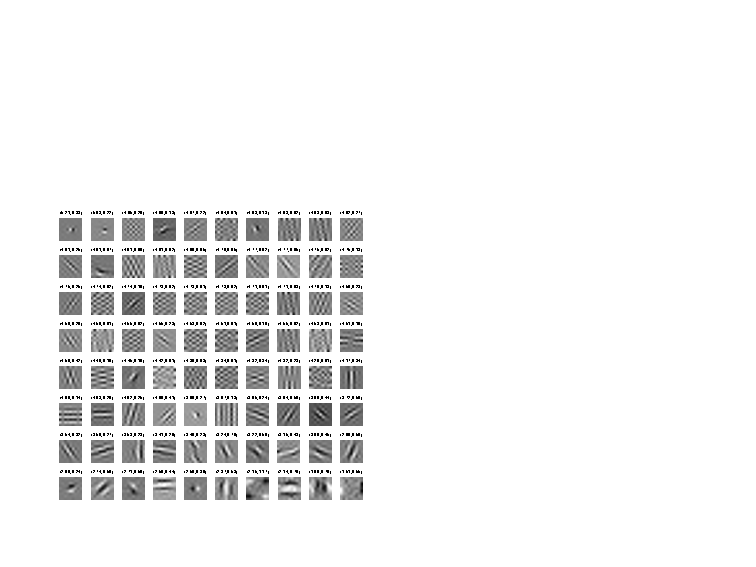
\includegraphics[height=0.5\textheight]{BilevelKernels}
  \par
  Learned kernels $k_i \colon \Domain \to \Real$.  
\end{column}
\begin{column}{0.45\textwidth}
  \centering
  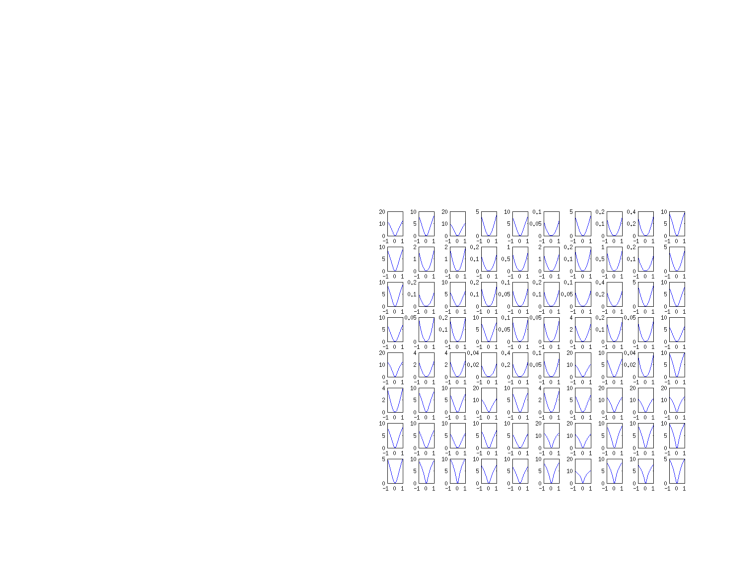
\includegraphics[height=0.5\textheight]{BilevelPotential}
  \par
  Potential functions $\rho_i \colon \Real \to \Real$.
\end{column}
\end{columns}
}
\onslide<7> % Slide 7
\structure{Sparse recovery (analysis formulation):} 
$\RegFunc_{\param}(\signal) := C\bigl( \rho_{\param}(\signal) \bigr)$ with $\param \subset \RecSpace$.
\begin{itemize}
  \item $C \colon \ell^2 \to \Real$ is a fix proper lower-semicontinuous function, e.g., $\ell^1$-norm.
  \item $\rho_{\param} \colon \RecSpace \to \ell^2$ analysis operator with $\param$ being the dictionary.  
  \item Denoising with $C =$ smooth version of $\ell^1$-penalty incl. proof that $\param \mapsto \model{\param}(\data)$ is differentiable: 
    \[ \model{\param}(\data) \in \argmin_{\signal} \Bigl[ \LogLikelihood\bigl( \ForwardOp(\signal),\data \bigr) + \RegFunc_{\param}(\signal) \Bigr] \]
    incl. explicit expression for the derivative (Theorem~1) \cite{Peyre:2011aa}.
  \item It is more common to consider the  synthesis (sparse coding) formulation, which we deal with in part related to `Sparse models'.
\end{itemize}
\end{overprint}
\end{frame}

% Frame
\begin{frame}{Summary of bi-level optimisation} 
\begin{itemize}
\item Computationally demanding due to implicit differentiation:
  \begin{itemize}
  \item For each $\param$, solve the inner problem 
    $\model{\param}(\data) \in \argmin_{\signal} \Bigl[ \LogLikelihood\bigl( \ForwardOp(\signal),\data \bigr) + \RegFunc_{\param}(\signal) \Bigr]$ exactly.
  \item Invert the Hessian of $\param \mapsto \model{\param}(\data)$.
  \end{itemize}
\item \structure{Alternative:} Unroll $T$ steps of an iterative algorithm (e.g. gradient descent):
  \vskip-0.25\baselineskip    
  \[ \begin{cases}
       \param^* \in \argmin_{\param} \Bigl[ \frac{1}{m} \sum_{i=1}^m \loss_{\RecSpace}\bigl(\model{\param,T}(\data_i),\signal_i\bigr) \Bigr] 
       & \\[1.5em]
       \signal_{\param}^{i+1} := \signal_{\param}^i - \omega_i \nabla\Bigl[ \LogLikelihood\bigl( \ForwardOp(\Cdot),\data \bigr) 
         + \RegFunc_{\param}(\Cdot) \Bigr](\signal_{\param}^i)
       & \text{ for $i=1,\ldots, T-1$} \\
       \model{\param,T}(\data) := \signal_{\param}^{T} &
    \end{cases} \]
  \vskip-0.5\baselineskip    
  \begin{itemize}
  \item Computing gradient of objective can be done efficiently.
  \item Taking only a few iterates ($T$ small) already works very well.
  \end{itemize}
\end{itemize}  
\end{frame}


% Frame
\begin{frame}{Incremental gradient scheme}
\begin{itemize} 
\item Assume you can decompose data log-likelihood and regularisation functional into $M$ components:
\vskip-\baselineskip
\[ \LogLikelihood\bigl( \ForwardOp(\signal),\data \bigr) = 
      \sum_{k=1}^M \LogLikelihood_k\bigl( \ForwardOp(\signal),\data \bigr)
   \quad\text{and}\quad
   \RegFunc_{\param}(\signal) := \RegFunc_0(\signal) + \sum_{k=1}^M \RegFunc_{\param_k}(\signal).
\]      
\vskip-\baselineskip
\item $\RegFunc_0$ typically non-smooth, e.g., handles additional sparsity priors or constraints.
\item \structure{Reconstruction method:} Let $F_k(\signal;\data,\param_k) := \LogLikelihood_k\bigl( \ForwardOp(\signal),\data \bigr) + \RegFunc_{\param_k}(\signal)$ and $i_k = \modulus(k,T)+1$, perform $T$ incremental proximal steps:
\[ \begin{cases}
     \signal_{\param}^{k+1} := \prox_{\omega_k \RegFunc_0}\bigl( \signal_{\param}^k - \omega_k \nabla F_{i_k}(\signal_{\param}^k; \data,\param_{i_k}) \bigr)
       & \text{for $k=1,\ldots, T-1$} \\[0.5em]
       \model{\param,T}(\data) := \signal_{\param}^{T} &
\end{cases}
\]   
\item Used for denoising and MRI reconstruction from under-sampled $k$-space data \cite{Kobler:2017aa,Hammernik:2018aa}.
\item Close connections to residual networks.
\end{itemize} 
\end{frame}


\begin{frame}{Example from 2D denoising}
 \begin{columns}[T]
\begin{column}{0.3\textwidth}
  \centering
  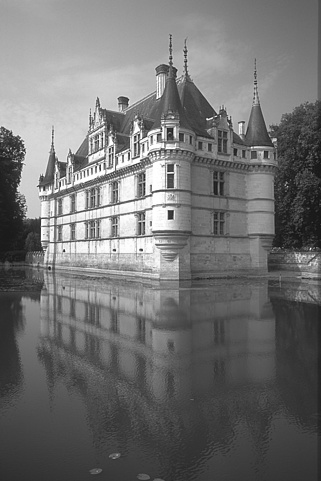
\includegraphics[height=0.8\textheight]{Original}
  \par
  Signal: True image
\end{column}
\begin{column}{0.3\textwidth}
    \centering
    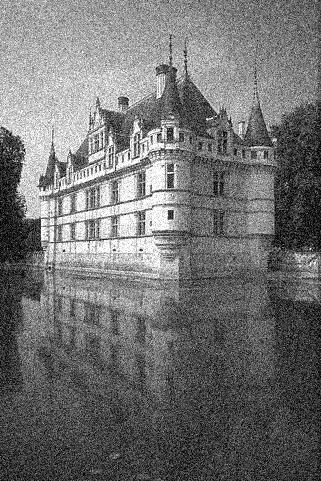
\includegraphics[height=0.8\textheight]{Data}
    \par Data: Noisy image.
\end{column}
\begin{column}{0.3\textwidth}
  \begin{overprint}
  \onslide<1>
    \centering
    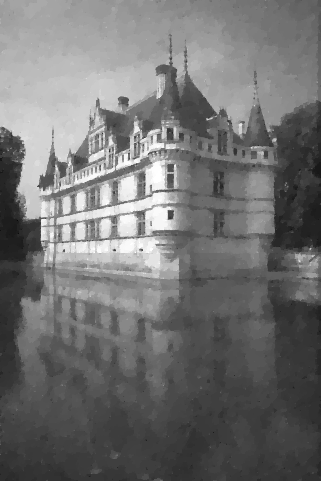
\includegraphics[height=0.8\textheight]{TV}
    \par Total variation.
  \onslide<2>
    \centering
    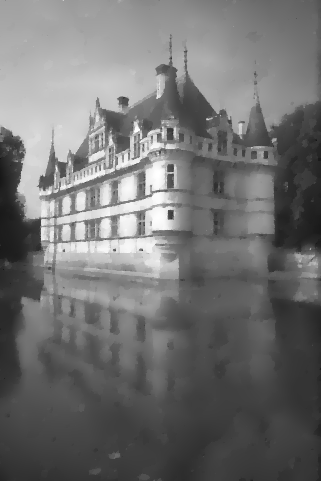
\includegraphics[height=0.8\textheight]{TGV2}
    \par TGV${}^2$.
  \onslide<3>
    \centering
    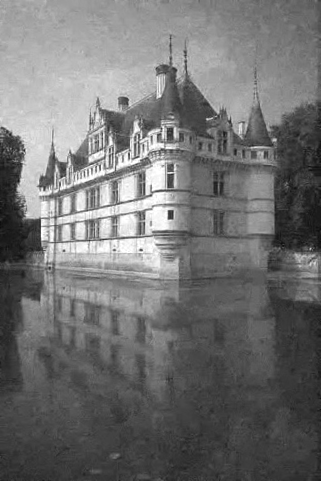
\includegraphics[height=0.8\textheight]{DCT5}
    \par Sparse dictionary (with DCT).
  \onslide<4>
    \centering
    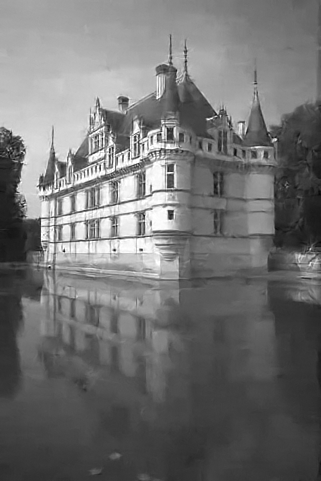
\includegraphics[height=0.8\textheight]{FoE}
    \par Nonconvex fields of experts.
  \onslide<5>
    \centering
    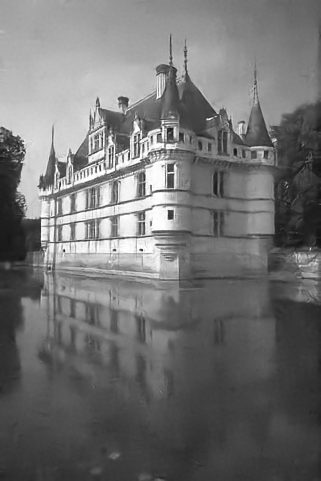
\includegraphics[height=0.8\textheight]{IDE}
    \par Incremental gradient scheme.
  \end{overprint}    
\end{column}
\end{columns}
\end{frame}

% Frame
\begin{frame}[plain]
\slideTitle{Sparse models}
\end{frame}

% Frame
\begin{frame}{Basic notions}
$\RecSpace$ separable Hilbert space (has countable ON-basis).
\begin{itemize}
\item \structure{Dictionary:} A collection $\Dict:=\{ \phi_i \}_i \subset \RecSpace$, elements are called atoms. Emerge from one of two sources \cite{Lanusse:2014aa,Bruckstein:2009aa,Rubinstein:2010aa,Chen:2016aa}:
  \begin{itemize}
  \item Analytic: Based on a mathematical model.
  \item Data-dependent: Derived from a set of realisations $\signal_i \in \RecSpace$.
  \end{itemize}
\item \structure{Frame:} $\Dict := \{ \phi_i \}_i$ is a frame if there exists $C_1,C_2 > 0$ such that 
  \[  C_1 \Vert \signal \Vert^2 
      \leq \sum_{i} \bigl\vert \langle \signal,\phi_i \rangle \bigr\vert^2 \leq 
      C_2 \Vert \signal \Vert^2
      \quad\text{for any $\signal \in \RecSpace$.}
  \]
\item \structure{Tight frame:} Case when $C_1=C_2=1$.
\item \structure{Over-complete/redundant:} The frame does \emph{not} form a basis for $\RecSpace$.
  Redundant dictionaries, e.g., translation invariant wavelets, often work better than non-redundant \cite{Peyre:2011aa,Elad:2010aa}.
\end{itemize}
\end{frame}

% Frame
\begin{frame}{Analysis and synthesis}
$\RecSpace$ separable Hilbert space, $\Dict := \{ \phi_i \}_i \subset \RecSpace$ fixed dictionary.
\begin{itemize}
\item \structure{Analysis operator:} $\AnOp \colon \RecSpace \to \ell^2$ where $\AnOp(\signal) := \bigl( \langle \signal,\phi_i \rangle \bigr)_i$
\item \structure{Synthesis operator:} $\SynthOp \colon \ell^2 \to \RecSpace$ is the adjoint of the analysis operator, i.e., 
  \[ \SynthOp\bigr((\gamma_i)_i\bigr) := \sum_i \gamma_i \phi_i. \]
\item \structure{Frame operator:} $\SynthOp \circ \AnOp \colon \RecSpace \to \RecSpace$, i.e.,
  \[ (\SynthOp \circ \AnOp)(\signal) = \sum_i \langle \signal,\phi_i \rangle \phi_i. \]
\end{itemize}
\end{frame}

% Frame
\begin{frame}{Notion of sparsity}
$\RecSpace$ separable Hilbert space, $\Dict := \{ \phi_i \}_i \subset \RecSpace$ fixed dictionary.
\begin{itemize}
\item \structure{Sparsity:} 
  $\signal \in \RecSpace$ is $s$-sparse w.r.t. $\Dict$ if 
  \[ \bigl\Vert \AnOp(\signal) \bigr\Vert_0 = \# \bigl\{ i \mid \langle \signal,\phi_i \rangle \neq 0 \bigr\} \leq s. \]
\item \structure{Compressible:} 
  $\signal \in \RecSpace$ is compressible w.r.t. $\Dict$ if the following power law decay holds:
  \[ \bigl\vert \widetilde{\AnOp}(\signal)_k \bigr\vert \leq C k^{-1/q}
     \quad\text{for some $C >0$ and $0 < q < 1$.}
 \]
 $\widetilde{\AnOp}(\signal) =$ a non-increasing rearrangement of the sequence $\AnOp(\signal)$.
\item Sparse signals are compressible.
  \par $q$ small $\implies$ compressibility = sparsity.
\item $\AnOp_s(\signal) =$ vector consisting of the $s$ largest (in magnitude) coefficients of the sequence $\AnOp(\signal)$.
\end{itemize}
\end{frame}


% Frame
\begin{frame}{Sparse recovery}{Problem formulation}
\begin{itemize}
\item \structure{Inverse problem:} Recover $\signaltrue \in \RecSpace$ from $\data = \ForwardOp(\signaltrue) + \datanoise$.
\item \structure{Data log likelihood:} $\LogLikelihood \colon \DataSpace \times \DataSpace \to \Real$.
\item \structure{Prior model:} $\signaltrue \in \RecSpace$ is compressible w.r.t. given dictionary $\Dict:=\{ \phi_i \}_i$.
\item \structure{Reconstruction method (sparse recovery)}
   \begin{itemize}
   \item Synthesis (sparse coding):
   \[
    \model{\param}(\data) := \SynthOp(\gamma^*)
    \quad\text{where}\quad
    \gamma^* \in \argmin_{\gamma \in \ell^2} 
      \Bigl[  \LogLikelihood\Bigl( \ForwardOp(\SynthOp(\gamma)), \data \Bigr) 
        + \param \alert<2-3>{\Vert} \gamma \alert<2-4>{\Vert_{\alt<4>{p}{0}}} 
      \Bigr].
    \]
  \item Analysis:
  \[
    \model{\param}(\data) \in \argmin_{\signal \in \RecSpace} 
      \Bigl[  \LogLikelihood\bigl( \ForwardOp(\signal), \data \bigr) 
        + \param \alert<2-4>{\bigl\Vert} \AnOp(\signal) \alert<2-4>{\bigr\Vert_{\alt<4>{p}{0}}}
      \Bigr].
  \]
  \end{itemize}
\item $\Dict$ is an ON basis $\implies$ synthesis and analysis formulations are equivalent. 
\visible<2->{\item Sparse recovery is \alert<1>{NP-hard}.}
\visible<3->{
\begin{itemize}
\item Greedy approach.
\item \alert<4>{Convex relaxation $p>0$}, case $p=1$ starting point for sparse signal processing \cite{Elad:2010aa,Foucart:2013aa}.
\end{itemize}
}
\end{itemize}
\end{frame}

% Frame
\begin{frame}{Sparse recovery}{Theory: Example of result}
\begin{block}{Theorem \cite{Candes:2006aa}}
Let $\RecSpace=\Real^n$, $\DataSpace=\Real^m$, and assume $\ForwardOp \colon \RecSpace \to \DataSpace$ be a linear 
mapping whose matrix satisfies the \alert<1-2>{restricted isometry property}. 
If $\data = \ForwardOp(\signaltrue) + \datanoise$ with 
$\Vert \datanoise \Vert \leq \delta$ and
\vskip-0.5\baselineskip
\[
\widehat{\signal}_{\delta} := \argmin_{\signal \in \RecSpace} \Vert \signal \Vert_1
\quad\text{subject to}\quad
\bigl\Vert \ForwardOp(\signal) - \data \bigr\Vert_2 \leq \delta,
\]
then 
\vskip-1.5\baselineskip
\[ \bigl\Vert \widehat{\signal}_{\delta} - \signaltrue \bigr\Vert_2 
     \leq C \biggl[ \alert<3>{\delta} + \frac{\alert<3>{\bigl\Vert \signaltrue - \signaltrue_s \bigr\Vert_2}}{\sqrt{s}} \biggr].
\]
$\signaltrue_s =$ vector consisting of the $s$ largest (in magnitude) coefficients of $\signaltrue$.
\end{block}
\vskip-0.25\baselineskip
\begin{overprint}
\onslide<1>
\structure{Restricted isometry property (RIP):} 
$\ForwardOp$ satisfies the following for sufficiently small $\epsilon_s>0$:
\vskip-0.25\baselineskip
\[ (1-\epsilon_s) \Vert \signal \Vert_2^2 
     \leq \bigl\Vert \ForwardOp(\signal) \bigr\Vert_2^2 \leq
   (1+\epsilon_s) \Vert \signal \Vert_2^2 
   \quad\text{for all $s$-sparse $\signal \in \RecSpace$.}
\]
RIP $\implies$ coherence (columns of $\ForwardOp$ are `uncorrelated').
\onslide<2>
\structure{Matrices satisfying RIP:} Sub-Gaussian matrices, partial bounded orthogonal matrices \cite{Chen:2016aa}.
\onslide<3>
\begin{itemize}
\item Reconstruction error is at most proportional to the norm of the \alert<3>{noise} in the data and the \alert<3>{tail} $\signaltrue - \signaltrue_s$ of the signal. 
\item Error bound is optimal (up to precise value of $C$) \cite{Cohen:2009aa}.
\item If $\signaltrue$ is $s$-sparse and $\delta=0$ (no noise) $\implies$ $\signaltrue$ can be reconstructed exactly.
\end{itemize}
\onslide<4>
\begin{itemize}
\item If $\signaltrue$ is compressible, then 
  \[ \bigl\Vert \widehat{\signal}_{\delta} - \signaltrue \bigr\Vert_2 
     \leq C \Bigl( \delta + C' s^{1/2-1/q} \Bigr).
  \]
\end{itemize}
\end{overprint}
\end{frame}

% Frame
\begin{frame}{Sparse recovery}{Solution methods}
\structure{Sparse coding:} Given dictionary $\{ \phi_i \}_i$, compute sparse representation 
\[
     \gamma^* \in \argmin_{\gamma \in \ell^2} 
      \biggl[  \Bigl\Vert \ForwardOp\Bigl( \sum_i \gamma_i \phi_i \Bigr) - \data \Bigr\Vert_2^2
        + \param \alt<2>{\Vert \gamma \Vert_{1}}{\Vert \gamma \Vert_{0}}
      \biggr].
\]
\begin{overprint}
\onslide<1>
\begin{itemize}
\item \structure{Greed approaches:} 
  Build up an approximation one step at a time by making locally optimal choices at each step.
  \begin{itemize}
  \item Iterative (hard) thresholding \cite{Blumensath:2008aa, Foucart:2016aa}. 
    \vskip-0.5\baselineskip
    \[ 
       \gamma^{i+1} = T_s\Bigl( \gamma^{i} - W^*\bigl( W(\gamma^{i}) - \data \bigr) \Bigr)
       \quad \text{where $W(\gamma) :=  \ForwardOp\Bigl( \sum_i \gamma_i \phi_i \Bigr)$.}
    \]
    \vskip-0.5\baselineskip
    $T_s(\gamma) =$ sets all but the largest (in magnitude) $s$ elements of $\gamma$ to zero.
    \par
    Proximal-gradient method with proximal of the function that is 0 at 0 and 1 everywhere else.
  \item Matching pursuit (MP) \cite{Mallat:1993aa}.
  \item Orthogonal matching pursuit (OMP) \cite{Tropp:2007aa} and variants like StOMP \cite{Donoho:2012aa}, 
   ROMP \cite{Needell:2009ab}, and CoSamp \cite{Needell:2009aa}.
  \end{itemize}
\end{itemize}
\onslide<2>
\begin{itemize}
\item \structure{Convex relaxation:}
  Most common example is to replace $\ell_0$-norm with $\ell_1$-norm
  $\implies$ Basis pursuit (BP) \cite{Candes:2006aa}, also called Lasso in the statistics literature \cite{Tibshirani:1996aa}.
  \begin{itemize}
  \item Interior-point methods \cite{Candes:2006ab,Kim:2007aa}.
  \item Projected gradient methods \cite{Figueiredo:2007aa}.
  \item Iterative soft thresholding (forward-backward/proximal-gradient, proximal operator of $\ell_1$ is sometimes called soft thresholding 
    operator) \cite{Fornasier:2008aa}.
  \item Iterative thresholding \cite{Daubechies:2004aa}.
  \item Fast proximal gradient methods (FISTA and variants) \cite{Bubeck:2015aa}.
  \end{itemize}
\end{itemize}
\onslide<3>
\begin{itemize}
\item \structure{Combinatorial algorithms:}
  Acquire highly structured samples of the signal that support rapid reconstruction via group testing. 
  This class includes Fourier sampling, chaining pursuit, and HHS pursuit, e.t.c. \cite{Berinde:2008aa}.
\end{itemize}
\onslide<4>
\begin{itemize}
\item Greedy methods will in general not give the same solution as convex relaxation. If the restricted nullspace property holds, then both 
  approaches have the same solution.
\item Convex relaxation: Succeed with a very small number of measurements, but they tend to be computationally burdensome.
\item Combinatorial algorithms: Extremely fast (sublinear in the length of the target signal) but they require very specific structure of $\ForwardOp$ and a large number of samples.
\item Greedy methods: Intermediate in their running time and sampling efficiency.
\end{itemize}
\end{overprint}
\end{frame}

\begin{frame}{Sparse recovery}{Patch-based local models}
\begin{itemize}
\item \structure{Patch-based local models:} Split signal into patches (segments), process patches.
\item Leading denoising methods are based on patch-based local models.
\begin{itemize}
\item K-SVD: Sparse coding of image patches \cite{Elad:2006aa}
\item BM3D: Combines sparsity and self-similarity \cite{Dabov:2007aa}
\item EPLL: Gaussian mixture model of the image patches \cite{Zoran:2011aa}
\item Deep \acp{CNN} \cite{Burger:2012aa}
\item NCSR: Non-local sparsity with centralised coefficients \cite{Dong:2013aa}
\item WNNM: Weighted nuclear norm regularisation of image patches \cite{Gu:2014aa}
\item SSC-GSM: Nonlocal sparsity with a Gaussian scale mixture \cite{Dong:2015aa}
\end{itemize}
\item \structure{Sparse-Land model:} Each patch is sparse w.r.t. some global dictionary, sparse coding applied patch-wise 
  \cite{Elad:2006ab,Dong:2011aa,Mairal:2014aa,Romano:2015aa,Sulam:2015aa}.
\item Computationally more feasible for dictionary learning.
\end{itemize}
\end{frame}

\begin{frame}{Sparse recovery}{Sparse-Land model: Setting}
\begin{columns}[T]
\begin{column}{0.39\textwidth}
\structure{Sparsity of patches}
\begin{itemize}
\item Dictionary: $\Dict = \{ \phi_k \}_k$
\item Patch: $\Patch_j(\signal) = \signal \vert_{\Omega_j}$ 
\item Model: Patches sparse in $\Dict$.
\item Patch-wise sparse coding:
  \vskip-0.25\baselineskip
  \[ \Patch_j(\signal) = \sum_{k} \gamma_{j,k} \phi_k \]
  \vskip-0.5\baselineskip
  $\gamma_{j,k} \approx 0$ for most $k$. 
\end{itemize}
\end{column}
\begin{column}{0.61\textwidth}
\structure{Illustration in discrete setting}
\begin{center}
\begin{tikzpicture}[      
        every node/.style={anchor=south west,inner sep=0pt},
        x=1mm, y=1mm,
      ]   
     \node (figure) at (0,0)
       {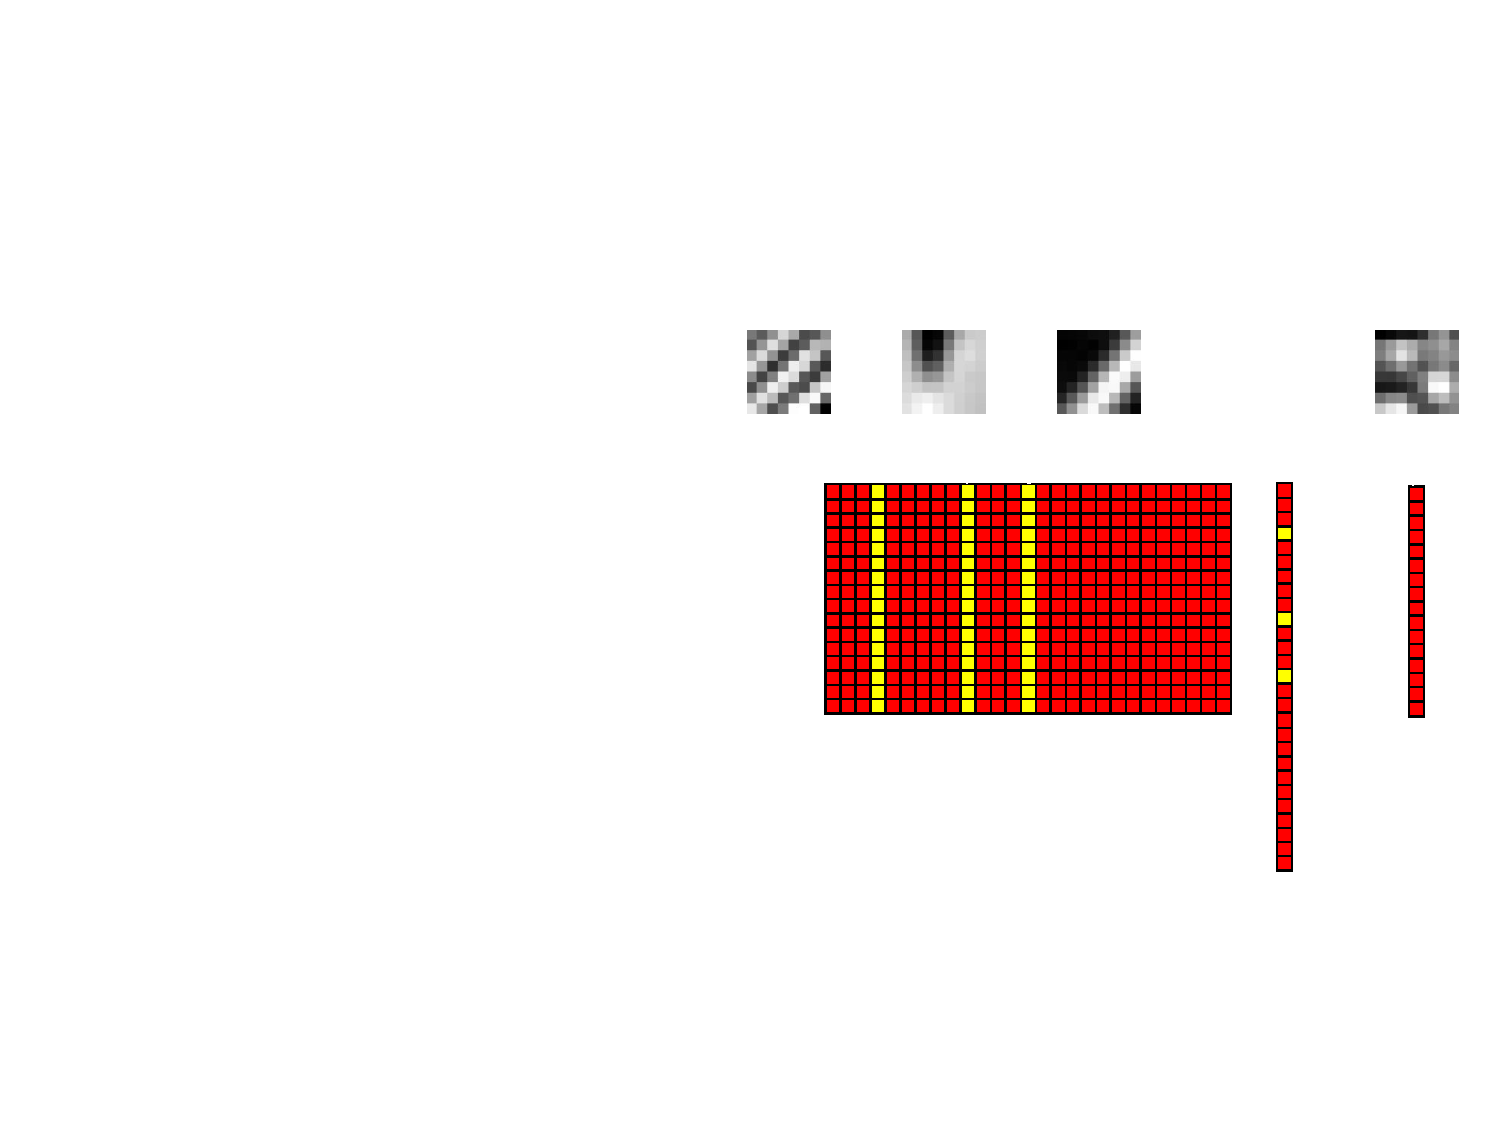
\includegraphics[height=0.7\textheight]{SparseLand_summary}};
     \put(155,70) {$=$}
     \put(132.5,70) {$\LogLikelihood$}
     \draw[red, <->,>=stealth] (8.5,15) -- (44.5,15) node[midway,below,yshift=-0.05cm,font=\scriptsize] {$m >n$};  % Horizontal arrow for dictionary
     \draw[red, <->,>=stealth] (7.25,16.7) -- (7.25,36.5) node[midway,left,xshift=-0.05cm,font=\scriptsize] {$n$};  % Vertical arrow for dictionary   
     \put(136,-5) {$\gamma_j$} % coefficients for i:th patch
     \put(165,30) {$\Patch_j(\signal)$} % i:th patch
     \put(50,20) {$\Dict= \{ \phi_k \}_k$} % Dictionary
     % Arrows pointing out dictionary elements
     \draw[red, ->,>=stealth] (13,37.2) -- (5.5,43);    
     \draw[red, ->,>=stealth] (21,37.2) -- (19,43);    
     \draw[red, ->,>=stealth] (26.5,37.2) -- (33,43);    
     % Arrow pointing out i:th patch
     \draw[red, ->,>=stealth] (62,37.2) -- (62,43);    
\end{tikzpicture}
\end{center}
\end{column}
\end{columns}
\end{frame}

\begin{frame}{Sparse recovery}{Sparse-Land model: Denoising}
\begin{itemize}
\item \structure{Inverse problem:} Recover $\signaltrue \in \RecSpace$ from $\data = \signaltrue + \datanoise$.
\item \structure{Data log likelihood:} $\LogLikelihood \colon \DataSpace \times \DataSpace \to \Real$.
\item \structure{Prior model (Sparse-Land model):} Given dictionary $\Dict \subset \RecSpace$ and $\Patch_j \colon \RecSpace \to \RecSpace$ (patch extraction operator) for $j=1,\ldots,N$, assume
  \[ \signaltrue = \sum_{j=1}^N \Patch_j(\signaltrue) 
     \quad\text{where $\Patch_j(\signaltrue) \in \RecSpace$ is compressible w.r.t. $\Dict$.}
  \]
\item \vskip-0.5\baselineskip
  Denoising:  
  \begin{itemize}
  \item Prior model can be applied to data $\implies \Patch_j(\data)$ compressible w.r.t. $\Dict$.
  \item Denoised patch: Given by synthesis $\SynthOp(\gamma_{j}^*) \in \RecSpace$ where $\gamma_{j}^* \in \ell^2$ solves sparse coding:
    \[ \gamma_{j}^* := 
          \argmin_{\gamma_j}  \Vert \gamma_j \Vert_0 
         \quad\text{subject to }
          \bigl\Vert \Patch_j(\data) - \SynthOp(\gamma_{j}) \bigr\Vert_2 \leq \epsilon.
     \]
   \item Denoised image: $\widehat{\signal} = \sum_j \SynthOp(\gamma_{j})$.
  \end{itemize}
\end{itemize}    
\end{frame}

\begin{frame}{Sparse recovery}{Sparse-Land model: Denoising}
\begin{overprint}
\onslide<1-4>
\begin{overlayarea}{\textwidth}{0.8\textheight}
\begin{columns}
\begin{column}{0.2\textwidth}
  \centering
  \visible<1->{
    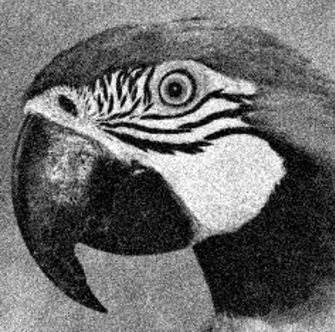
\includegraphics[width=\textwidth]{noisy_image}
  }
\end{column}
\hfill \visible<2->{{\Huge $\Rightarrow$}} \hfill
\begin{column}{0.2\textwidth}
  \centering
  \visible<2->{
  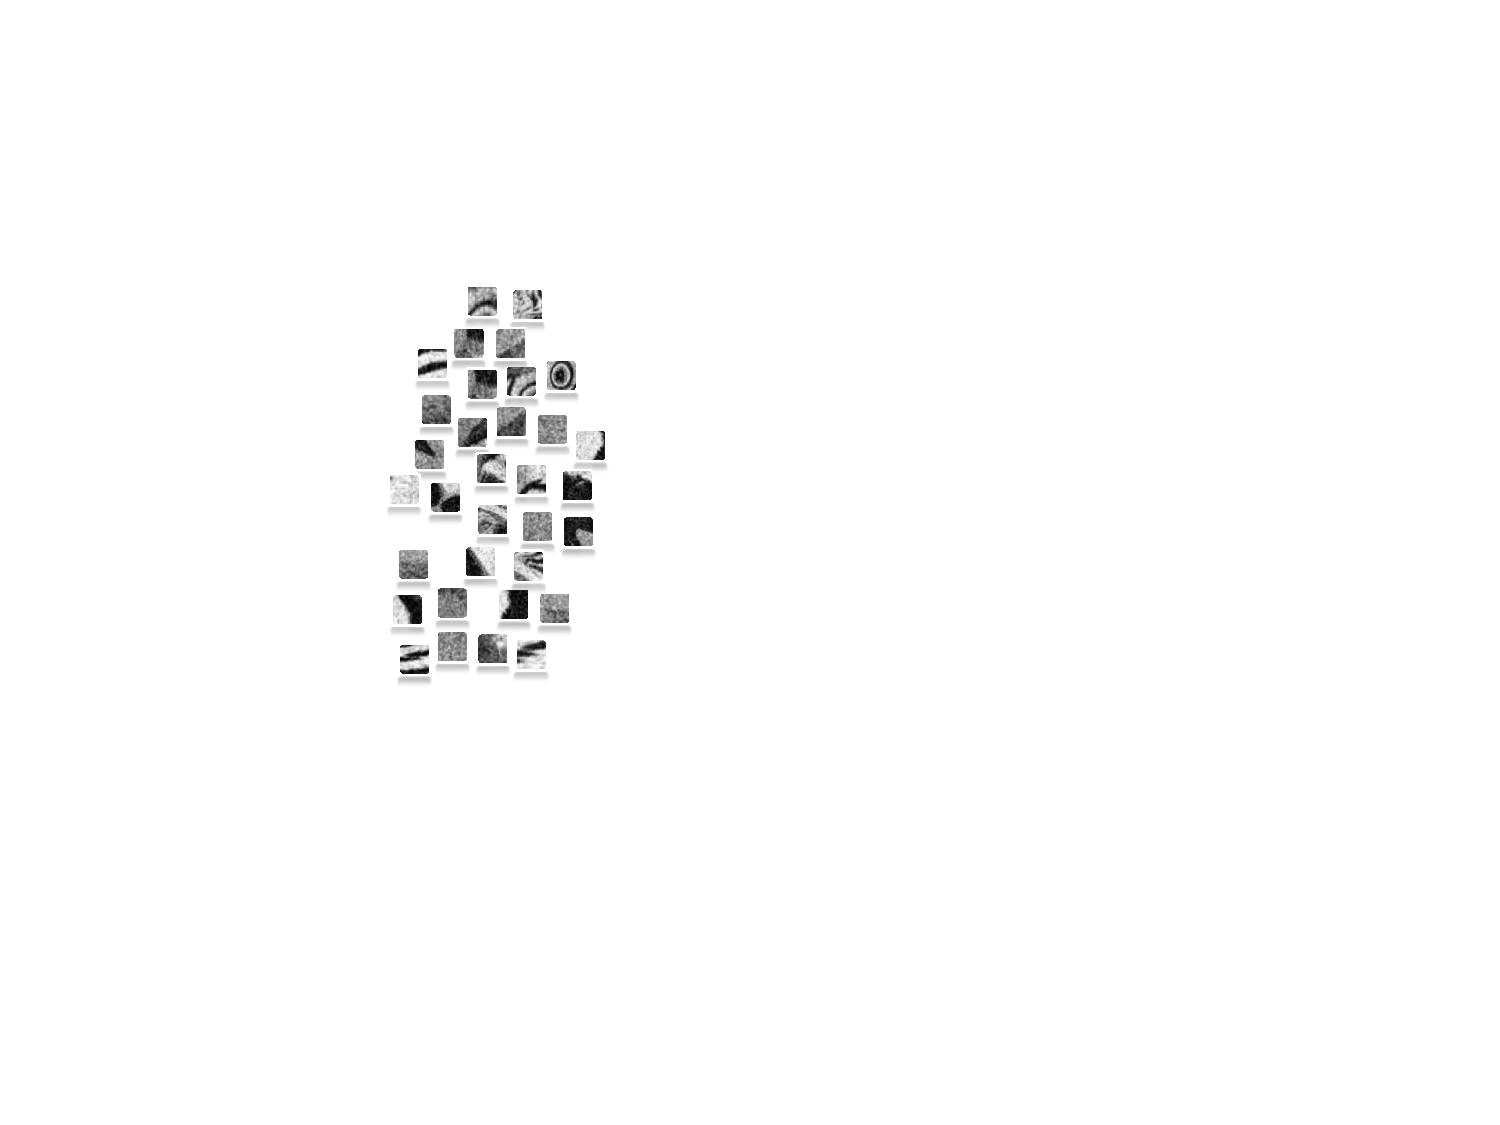
\includegraphics[width=\textwidth]{patches_noisy}
  }
\end{column}
\hfill \visible<3->{{\Huge $\Rightarrow$}} \hfill
\begin{column}{0.2\textwidth}
  \centering
  \visible<3->{
  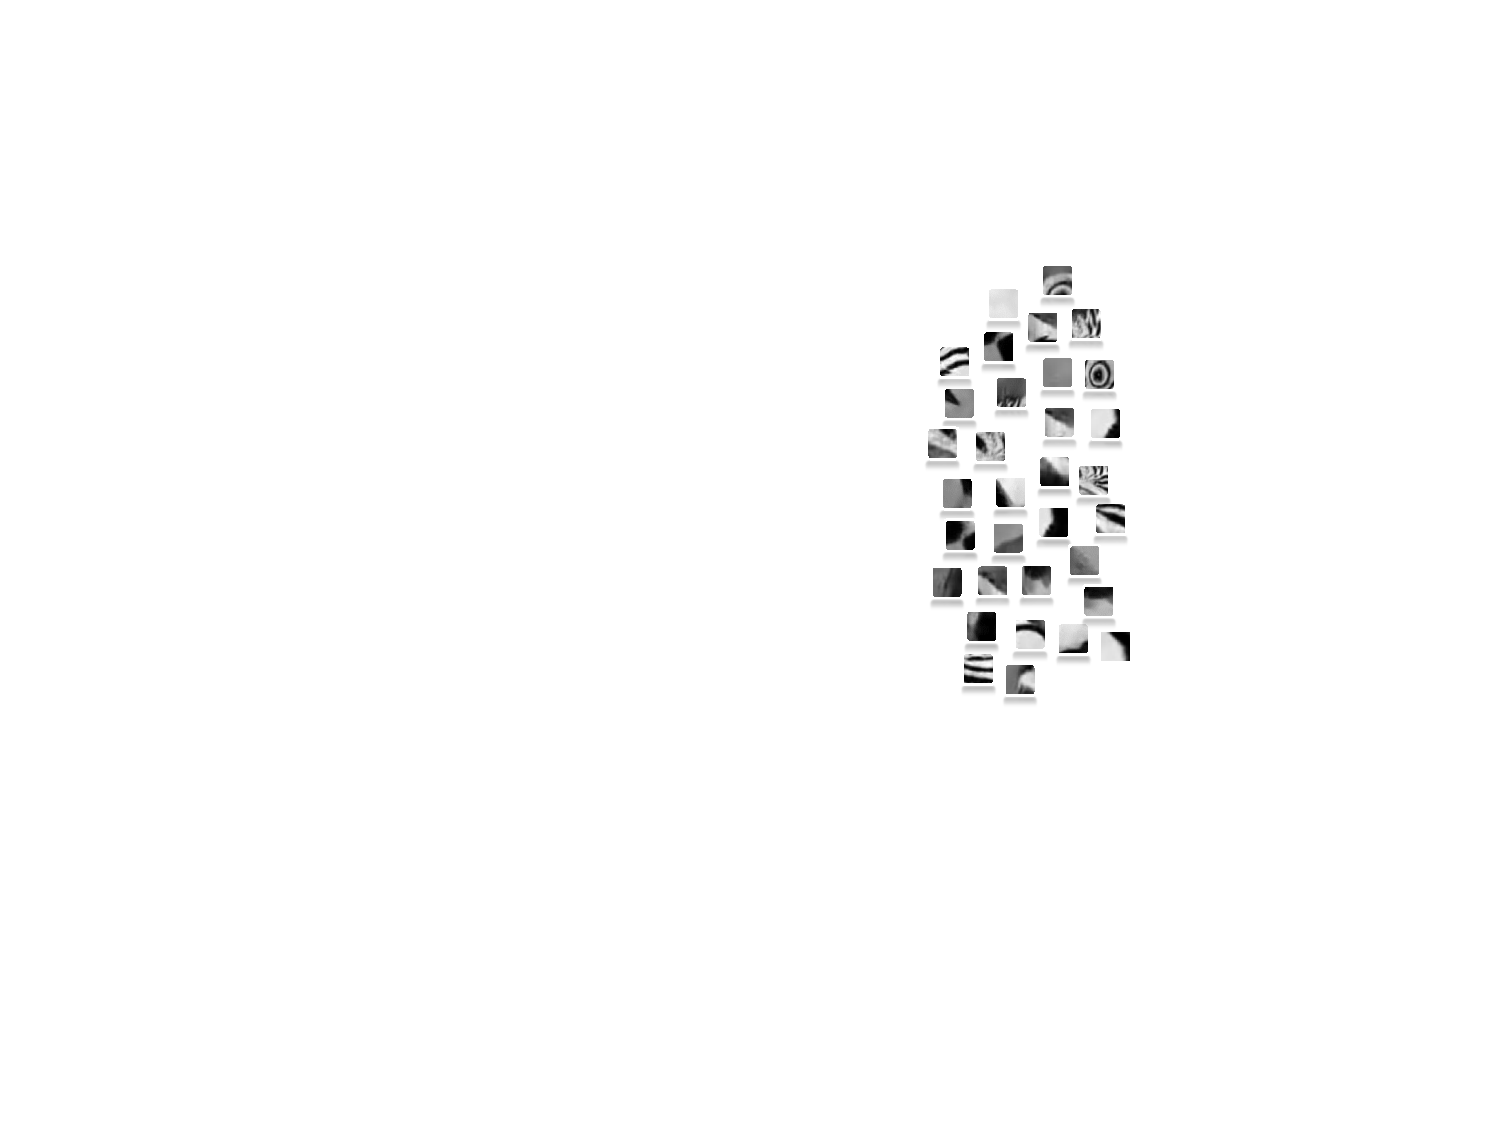
\includegraphics[width=\textwidth]{patches_denoised}
  }
\end{column}
\hfill \visible<4->{{\Huge $\Rightarrow$}} \hfill
\begin{column}{0.2\textwidth}
  \centering
  \visible<4->{
  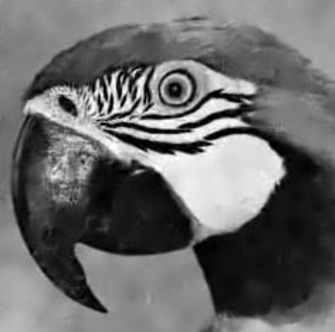
\includegraphics[width=\textwidth]{original_image}
  }
\end{column}
\end{columns}
\end{overlayarea}
\end{overprint}
\end{frame}

\begin{frame}{Sparse recovery}{Sparse-Land model: Example approaches for general inverse problems}
\structure{Global dictionary based statistical iterative reconstruction (GDSIR)}
\begin{itemize}
\item \structure{Inverse problem:} Recover $\signaltrue \in \RecSpace$ from $\data = \ForwardOp(\signaltrue) + \datanoise$.
\item \structure{Prior model:} Sparse-Land model with $N$ patches w.r.t. given dictionary $\Dict \subset \RecSpace$ and associated synthesis operator 
  $\SynthOp \colon \ell^2 \to \RecSpace$. 
\item \structure{Reconstruction method:} 
\alt<2>{Intertwined scheme \cite{Bai:2017aa}:}{No sense to divide data into patches, instead}
\begin{overprint}
\onslide<1>
\vskip-0.5\baselineskip
\[ \min_{\signal \in \RecSpace, \gamma_i \in \ell^2}
     \Bigl[ 
       \LogLikelihood\bigl(\ForwardOp(\signal),\data\bigr) + \RegFunc_{\param}(\signal,\gamma_1,\ldots, \gamma_N)
     \Bigr]
\]     
where  
\[ \RegFunc_{\param}(\signal,\gamma_1,\ldots, \gamma_N) 
     := \sum_{j=1}^N 
            \Bigl[
              \lambda_j \bigl\Vert \Patch_j(\signal) - \SynthOp(\gamma_j) \bigr\Vert_2^2 + \mu_j \Vert \gamma_j \Vert_p^p
            \Bigr] 
\]     
with $\param = (\lambda_j, \mu_j)_{j=1}^N \in (\Real^{2})^N$.
\onslide<2>
\[ \begin{cases}
    \signal^{i+1} := \argmin_{\signal \in \RecSpace}
    \biggl[ 
       \LogLikelihood\bigl(\ForwardOp(\signal),\data\bigr)
       + \sum_{j=1}^N \lambda_j
            \Bigl[
              \bigl\Vert \Patch_j(\signal) - \SynthOp(\gamma^i_j) \bigr\Vert_2^2
            \Bigr] 
     \biggr]
    &\\
    \gamma_j^{i+1} := \argmin_{\gamma \in \ell^2}
    \biggl[ 
       \lambda_j \bigl\Vert \Patch_j(\signal^{i+1}) - \SynthOp(\gamma_j) \bigr\Vert_2^2 + \mu_j \Vert \gamma_j \Vert_p^p 
    \biggr] 
    \quad\text{for $j=1,\ldots, N$.}  
    &      
\end{cases}\]
\end{overprint}
\end{itemize}
\end{frame}

\begin{frame}{How to find the dictionary?}
\begin{itemize}
\item \alert<1>{Determine jointly while performing reconstruction (joint reconstruction \& dictionary learning).}
\item Specify analytically.
\item Determine from example data (dictionary learning).
\end{itemize}
\end{frame}


\begin{frame}{Joint reconstruction \& dictionary learning}{Example of approach}
\structure{Adaptive dictionary based statistical iterative reconstruction (ADSIR)}
\begin{itemize}
\item \structure{Inverse problem:} Recover $\signaltrue \in \RecSpace$ from $\data = \ForwardOp(\signaltrue) + \datanoise$.
\item \structure{Prior model:} Sparse-Land model as in GDSIR.
\item \structure{Reconstruction method:} 
  Adds dictionary $\Dict = \{ \phi_i \}_i \subset \RecSpace$ as variable to GDSIR \cite{Xu:2012aa}, see also \cite{Chun:2017aa}.
 \[ \min_{\substack{\signal \in \RecSpace \\ \gamma_i \in \ell^2,\Dict \subset \RecSpace}}
     \Bigl[ 
       \LogLikelihood\bigl(\ForwardOp(\signal),\data\bigr) + \RegFunc_{\param}(\signal,\gamma_1,\ldots, \gamma_N, \Dict)
     \Bigr]
  \]     
  where
\[ \RegFunc_{\param}(\signal,\gamma_1,\ldots, \gamma_N,\Dict) 
     := \sum_{j=1}^N 
            \Bigl[
              \lambda_j \bigl\Vert \Patch_j(\signal) - \SynthOp_{\Dict}(\gamma_j) \bigr\Vert_2^2 + \mu_j \Vert \gamma_j \Vert_p^p
            \Bigr] 
\]     
with $\param = \bigl( (\lambda_j, \mu_j), \Dict) \in (\Real^{2})^N \times \RecSpace$ and $\SynthOp_{\Dict} \colon \ell^2 \to \RecSpace$ denotes synthesis operator associated with the dictionary $\Dict$.
\item Alternating minimisation scheme is used to optimise the three variables.
\end{itemize}
\end{frame}

\begin{frame}{How to find the dictionary?}
\begin{itemize}
\item Determine jointly while performing reconstruction (joint reconstruction \& dictionary learning).
\item Specify analytically.
\item \alert<1>{Determine from example data (dictionary learning).}
\end{itemize}
\end{frame}


\begin{frame}{Dictionary learning}
\begin{itemize}
\item \structure{Setting:}
  \begin{itemize}
  \item $\loss_{\RecSpace} \colon \RecSpace \times \RecSpace \to \Real$ loss function, e.g., 2- or 1-norm.
  \item Unsupervised training data $\signal_1, \ldots, \signal_N \in \RecSpace$.
  \item Dictionary $\Dict := \{ \phi_k \}_k \subset \RecSpace$.
  \item Synthesis operator $\SynthOp_{\Dict} \colon \ell^2 \to \RecSpace$ given as $\SynthOp_{\Dict}(\gamma) = \sum_k \gamma_k \phi_k$ for $\gamma \in \ell^2$.
  \end{itemize}
\end{itemize}
\vskip-0.5\baselineskip
\begin{overprint}
\onslide<1>
\begin{itemize}  
\item \structure{Dictionary learning (sparsity requirement):} 
    \[ \begin{cases}
      \argmin_{\substack{\gamma_i \in \ell^2 \\ \Dict \subset \RecSpace}}\,
        \sum_{i=1}^N \loss_{\RecSpace}\bigl(\signal_i, \SynthOp_{\Dict}(\gamma_i) \bigr)
      & \\[1.75em]
      \Vert \gamma_i \Vert_0 \leq s \text{ for $i=1,\ldots,N$.} &
      \end{cases}
      \quad\text{for given sparsity level $s$.}
    \]
\end{itemize}
\onslide<2>
\begin{itemize}  
\item \structure{Dictionary learning (precision requirement):}  
  \[ \begin{cases} 
     \argmin_{\substack{\gamma_i \in \ell^2 \\ \Dict \subset \RecSpace}}\,
      \sum_{i=1}^N \Vert \gamma_i \Vert_0
      & \\[1.75em]
     \loss_{\RecSpace}\bigl(\signal_i, \SynthOp_{\Dict}(\gamma_i) \bigr) \leq \epsilon \text{ for $i=1,\ldots,N$.}&
   \end{cases}
   \quad\text{for given precision $\epsilon>0$.}
  \]
  Objective is total cost for representing signals in training data w.r.t. a dictionary.
\end{itemize}
\onslide<3->
\begin{itemize}  
\item \structure{Dictionary learning (unified formulation):}
\vskip-0.5\baselineskip
\[ \argmin_{\substack{\gamma_i \in \ell^2 \\ \Dict \subset \RecSpace}}\,
      \alert<6>{\sum_{i=1}^N} \biggl[ \loss_{\RecSpace}\bigl(\signal_i, \SynthOp_{\Dict}(\gamma_i) \bigr) + \param \alert<4-5>{\Vert} \gamma_i \alert<4-5>{\Vert_{\alt<5>{1}{0}}} \biggr]
\]
\vskip-\baselineskip
\visible<4->{\item All formulations are NP-hard} \visible<5->{$\implies$ Convex relaxation.}
\visible<6->{\item \alert<6>{Fix} $\alert<6>{\Dict} \implies$ \alert<6>{sum} in objective \alert<6>{decouples} $\implies$ \alert<6>{sparse coding}:
\vskip-0.5\baselineskip
\[ \gamma^*_i := \argmin_{\gamma \in \ell^2}\,
      \biggl[ \loss_{\RecSpace}\bigl(\signal_i, \SynthOp_{\Dict}(\gamma) \bigr) + \param \Vert \gamma \Vert_{1} \biggr]
    \quad\text{for $i=1,\ldots, N$.}
\]
}
\end{itemize}
\end{overprint}
\end{frame}

\begin{frame}{Dictionary learning}{Finite dimensional setting}
\begin{itemize}
\item \structure{Setting:}
  \begin{itemize}
  \item $\RecSpace=\Real^n$ and $\ell^2$ replaced by $\Real^m$ for some $m$.
  \item Dictionary: $\Dict := \{ \phi_k \}_{k=1}^m \subset \Real^n$ represented by $(n \times m)$-matrix $\DictMat$
    \par $\implies$ synthesis operator $\SynthOp_{\DictMat} \colon \Real^m \to \Real^n$ with 
    $\SynthOp_{\DictMat}(\gamma) = \DictMat \cdot \gamma$.
  \alt<1>{%
    \item Dictionary size $m$ can be larger than $n$ to exploit redundancy.  
    \par $\DictMat$ is a basis $\implies$ unique solution (good) but limited expressiveness (bad). 
    \par $\DictMat$ overcomplete $\implies$ multiple solutions (bad) but greater expressiveness (good).
    }{}
  \end{itemize}
\item \structure{Dictionary learning (unified formulation):}
\[ \min_{\substack{\gamma_i \in \Real^m \\ \DictMat \in \Real^{n \times m}}}\,
      \sum_{i=1}^N \biggl[ \loss_{\RecSpace}\bigl(\signal_i, \DictMat \cdot \gamma_i \bigr) + \param \Vert \gamma_i \Vert_{1} \biggr].
\]
\visible<2->{
\item Simultaneously learn dictionary $\DictMat$ and sparse representation $\GammaMat := [ \gamma_1 \ldots \gamma_N ]$.
}
\visible<3->{
\item $\DictMat$ satisfies RIP $\implies$ relaxation preserves sparse solution \cite{Candes:2006aa}.
\item Separately convex in $\DictMat$ and $\GammaMat$, but not jointly convex
  \par $\implies$ intertwined iterates that alternatingly update $\DictMat$ and $\GammaMat$.
\item Fixed $\DictMat \implies$ sparse coding problem.
}
\end{itemize}
\end{frame}

\begin{frame}{Dictionary learning}
\structure{Problem:} Simultaneously learn dictionary $\DictMat$ and sparse representation $\gamma_i$'s using $L^2$-loss:
\[ \min_{\substack{\gamma_i \in \Real^m \\ \DictMat \in \Real^{n \times m}}}\,
      \sum_{i=1}^N \biggl[ \bigl\Vert \signal_i - \DictMat \cdot \gamma_i \bigr\Vert_2^2 + \param \Vert \gamma_i \Vert_{1} \biggr].
\]
\begin{overprint}
\onslide<1>
\begin{itemize}
\item Intertwined alternated updating of (matrices) $\DictMat$ and $\GammaMat := [ \gamma_1 \ldots \gamma_N ]$. 
\item State-of-the-art dictionary learning algorithms \cite{Rubinstein:2010aa}:
  \begin{itemize}
  \item K-SVD \cite{Aharon:2006aa}: Two-stage iterative process. 
  \item Geometric multi-resolution analysis (GRMA) \cite{Allard:2012aa}.
  \item Online dictionary learning \cite{Mairal:2010aa}.
  \end{itemize}
\item Most work done in the context of denoising.
\end{itemize}
\onslide<2>
\structure{K-SVD} \cite{Aharon:2006aa}: Two-stage iterative process. 
\begin{itemize}
\item Sparse coding stage: Solve a sparse coding problem to compute a sparse representation with a priori bound on sparsity.
\item Codebook update stage: Sequentially changes dictionary atoms (columns of $\DictMat$) and update relevant 
  $\gamma_i$'s (coefficients of the sparse representation).
\end{itemize}
\onslide<3>
\structure{Geometric multi-resolution analysis (GRMA)} \cite{Allard:2012aa}:
\begin{itemize}
\item Training data are noisy samples from a probability distribution on $n_0$-dimensional manifold $M \subset R^n$ where $n_0 \ll n$.
\item Analyse $M$ by techniques from geometric measure theory \cite{Jones:1990aa,David:1993aa} and multi-scale approximation 
  \cite{Binev:2004aa,Binev:2005aa}.
\item Resulting dictionary (geometric wavelets) is structured in a multi-scale fashion with synthesis and analysis operators that can be computed fast.
\end{itemize}
\onslide<4>
\structure{Online dictionary learning} \cite{Mairal:2010aa}:
\begin{itemize}
\item Randomly sample the training set.
\item Use at each iteration only one sample to update the dictionary. 
\item Shown to be significantly faster than batch algorithms while achieving similar results.
\end{itemize}
\end{overprint}
\end{frame}


\begin{frame}{Convolutional dictionaries}
\begin{itemize}
\item Issues with the Sparse-Land model: 
  \begin{enumerate}
  \item Performing sparse coding over all the patches tends to be a slow process.
  \\[0.5em]
  Can be addressed using learned iterative scheme, e.g., LISTA which learns a finite number of unrolled ISTA iterates using 
  unsupervised training data as to match ISTA solutions \cite{Gregor:2010aa}.
  \\[0.75em]
  \item Learning a dictionary over each patch independently cannot account for global information, e.g., shift-invariance in images.
  \\[0.5em]
  Need computational feasible approach that introduces further structure and invariances on dictionary, e.g., shift-invariance and 
  making each atom dependent on whole signal instead of patches.
  \end{enumerate}
\visible<2->{  
\item \structure{Convolutional dictionaries:}
  Atoms given by convolutional kernels and act on signal features by convolutions, i.e., $\DictMat$ is a concatenation of Toeplitz matrices (union of banded and circulant matrices).
  \par $\implies$ Computationally feasible shift-invariant dictionary where atoms depend on entire signal.
}  
\end{itemize}
\end{frame}

\begin{frame}{Convolutional Sparse Model}{Sparse coding}
\begin{itemize}
\item \structure{Inverse problem:} Recover $\signaltrue \in \RecSpace$ from $\data = \ForwardOp(\signaltrue) + \datanoise$.
\item \structure{Data log likelihood:} $\LogLikelihood \colon \DataSpace \times \DataSpace \to \Real$.
\item \structure{Prior model:} $\signaltrue \in \RecSpace$ is compressible w.r.t. convolution dictionary $\Dict:=\{ \phi_i \}_i \subset \RecSpace$.
\item \structure{Convolutional Sparse Coding (CSC):} Sparse coding (synthesis) using convolutional dictionaries (atoms act by convolutions):
   \[
    \model{\param}(\data) := \sum_i \gamma_i^* \ast \phi_i
    \quad\text{where}\quad
    \gamma_i^* \in \argmin_{\gamma_i \in \RecSpace} 
      \Bigl[  \LogLikelihood\Bigl( \ForwardOp\Bigl(\sum_i \gamma_i \ast \phi_i\Bigr), \data \Bigr) 
        + \param \sum_i \Vert \gamma \Vert_{0} 
      \Bigr].
    \]  
\item Methods for denoising by CSC use convex relaxation followed by ADMM in frequency space \cite{Bristow:2013aa}, along with variants of it.
 See als \cite{Sreter:2017aa} for using LISTA in this context.
\item Analysed in the context of denoising \cite{Bristow:2013aa,Wohlberg:2014aa,Gu:2015aa,Papyan:2016aa,Papyan:2016ab,Garcia-Cardona:2017aa}.
\item Theoretical properties for denoising analysed in \cite{Papyan:2016aa,Papyan:2016ab}.
\end{itemize}
\end{frame}

\begin{frame}{Convolutional Sparse Model}{Dictionary learning}
\begin{itemize}
\item Unsupervised training data: $\signal_1,\ldots, \signal_N \in \RecSpace$.
\item Loss function $\loss_{\RecSpace} \colon \RecSpace \to \RecSpace$.
\item Convolutional dictionary learning: 
\[    \min_{\phi_{i}, \gamma_{j,i} \in \RecSpace}\, 
      \biggl[  \sum_{j=1}^N \loss_{\RecSpace}\Bigl( \signal_j, \sum_i \gamma_{j,i} \ast \phi_{i} \Bigr)
          + \param \sum_{j=1}^N \sum_i \Vert \gamma_{j,i} \Vert_{1}
      \biggr]
      \quad\text{and $\Vert \phi_{i} \Vert_2=1$.}
\]  
\item Convex relaxation and $L^2$-loss: Solved using ADMM type of scheme \cite{Garcia-Cardona:2017aa}.
\item Extension to supervised data setting: Learn discriminative dictionaries instead of purely reconstructive ones by
  introducing a supervised regularisation term into the usual CSC objective that encourages the final dictionary elements to 
  be discriminative \cite{Affara:2018aa}.
\end{itemize}
\end{frame}

\begin{frame}{Multi-Layer Convolutional Sparse Model}
\structure{Multi-Layer Convolutional Sparse Model (ML-CSC)} \cite{Sulam:2017aa}
\begin{itemize}
\item $L$ convolution dictionaries $\Dict_1, \ldots, \Dict_L \subset \RecSpace$.
\item \structure{Prior model:} 
  \begin{itemize}
  \item $\signaltrue \in \RecSpace$ is compressible w.r.t. convolution dictionary $\Dict_1:=\{ \phi_{1,i} \}_i \subset \RecSpace$.
  \item Atoms $\phi_{k,i} \in \Dict_k$ are compressible w.r.t. convolution dictionary $\Dict_{k+1}$ for $k=1,\ldots,L-1$.
  \end{itemize}
\item Special case of a Convolutional Sparse Model where intermediate representations have specific structure \cite[Lemma~1]{Sulam:2017aa}.
\item Building on theory for CSC, \cite{Sulam:2017aa} provides a theoretical study of this novel model and its associated 
  pursuits for dictionary learning and sparse coding (for denoising).
  \par $\implies$ Layered thresholding algorithm and the layered basis pursuit which share many similarities with deep \acp{CNN}. 
\end{itemize}
\end{frame}

\begin{frame}{Multi-Layer Convolutional Sparse Model}{Connection to deep \ac{CNN}}
\structure{Theoretical analysis of ML-CSC} \cite{Papyan:2017aa}.
\begin{itemize}
\item ML-CSC yields a Bayesian model implicitly imposed on $\signaltrue$ when deploying a \ac{CNN}
  \par $\implies$ Characterise signals belonging to the model behind a deep \ac{CNN}.
\item Does not assume any specific property of network's parameters (apart from broad coherence).
  \begin{itemize}
  \item \cite{Bruna:2013aa,Mallat:2016aa} assumes filters are Wavelets.
  \item \cite{Giryes:2015aa} assumes random weights.
  \end{itemize}
\end{itemize}

\end{frame}
\begin{frame}{Multi-Layer Convolutional Sparse Model}{Connection to deep \ac{CNN}}
\structure{Theoretical analysis of ML-CSC} \cite{Papyan:2017aa}.
\begin{itemize}
\item Deep \ac{CNN} $\iff$ layered thresholding algorithm.
\item Offers a mathematical analysis of the \ac{CNN} architecture:
  \begin{itemize}
  \item Theorem~4: The \ac{CNN} is guaranteed to recover an estimate of the underlying representations of an input signal, 
    assuming these are sparse in a local sense.
  \item Theorem~8 \& 10: Adding norm-bounded noise to the signal results in a bounded perturbation in the output
    $\implies$ stability of the \ac{CNN} in recovering the underlying representations.
  \end{itemize}
\item ML-CSC can be used to propose an alternative to the commonly used forward pass algorithm in \ac{CNN}.
  This is related to both deconvolutional \cite{Zeiler:2010aa,Pu:2016aa} and recurrent networks \cite{Bengio:1994aa}.
\item Many of the results also hold for fully connected networks.
\end{itemize}
\end{frame}

\begin{frame}{Deep Dictionary Learning}
\begin{itemize}
\item Two popular representation learning paradigms: Dictionary learning and deep learning. 
  \begin{itemize}
  \item Dictionary learning focuses on learning `basis' and `features' by matrix factorisation.
  \item Deep learning focuses on extracting features via learning `weights' or `filter' in a greedy layer by layer fashion. 
\end{itemize}
\item Deep dictionary learning: Deeper architectures are built using the layers of dictionary learning \cite{Tariyal:2016aa}.
\item Competitive against other deep learning approaches, such as stacked autoencoder, deep belief network, and convolutional neural network, 
  regarding  classification and clustering accuracies. 
\end{itemize}
\end{frame}

%\begin{frame}{Prior model}{Other}
%\cite{Chun:2018aa}
%Convolutional analysis operator learning (CAOL): 
%earning kernels has mostly relied on so-called local approaches that extract and store many overlapping patches across training signals. Due to memory demands, local approaches have limitations when learning kernels from large datasets -- particularly with multi-layered structures, e.g., convolutional neural network (CNN) -- and/or applying the learned kernels to high-dimensional signal recovery problems. The so-called global approach has been studied within the "synthesis" signal model, e.g., convolutional dictionary learning, overcoming the memory problems by careful algorithmic designs. The CAOL is a framework in the global approach, and develops a new convergent Block Proximal Gradient method using a Majoriser to solve the corresponding block multi-nonconvex problems. To learn diverse filters within the CAOL framework, this paper introduces an orthogonality constraint that enforces a tight-frame filter condition, and a regulariser that promotes diversity between filters
%\end{frame}

% Frame
\begin{frame}[plain]
\slideTitle{Other}
\end{frame}


\begin{frame}{Prior with black box denoiser}
\begin{itemize}
\item There is an abundance of high-performing image denoising algorithms, would be nice to integrate these in reconstrruction.
\item Design regularisation that can incorporate a black box denoiser?
\end{itemize}
\vskip-0.75\baselineskip
\begin{overprint}
\onslide<1>
\begin{itemize}
\item \structure{Plug-and-Play Prior (P${}^3$) method} \cite{Venkatakrishnan:2013aa}
  \begin{itemize}
  \item Implicit prior for regularising general inverse problems. 
  \item Based on using the ADMM optimisation scheme: The overall problem decomposes into a sequence of image denoising tasks, 
    coupled with simpler $L^2$-regularised inverse problems that are much easier to handle.
  \item Regularisation only implicitly implied by the denoising algorithm
    \par $\implies$ No clear definition of the objective function (unclear if there is an underlying objective function).
  \item Stability issues, parameter tuning of the ADMM scheme is a delicate matter.
  \item Intimately coupled with the ADMM algorithm, does not offer easy and flexible ways of replacing the iterative procedure.
  \end{itemize}
\end{itemize}
\onslide<2>
\begin{itemize}
\item \structure{Regularisation by Denoising (RED)} \cite{Romano:2017aa} 
\begin{itemize}
\item \structure{Reconstruction method:}
  \[  
    \min_{\signal \in \RecSpace} \bigl[ \LogLikelihood\bigl(\ForwardOp(\signal), \data\bigr) + \RegFunc_{\param}(\signal) \bigr]
    \quad\text{with}\quad
    \RegFunc_{\param}(\signal) := \param \bigl\langle \signal, \signal - \Lambda(\signal) \bigr\rangle
  \]
  and where $\Lambda \colon \RecSpace \to \RecSpace$ is denoiser.
\item Denoiser needs to fulfil some weak conditions (local homogeneity and strong passivity).
  $\implies$ Can efficiently compute gradient of denoiser
\item Many Denoising algorithms, such as the NLM, kernel-regression, K-SVD, fulfil necessary assumptions.
\item More general, simpler and stabler alternative to the P${}^3$ method.
\end{itemize}
\end{itemize}
\end{overprint}  
\end{frame}

\begin{frame}[t, allowframebreaks]
\frametitle{References}
\bibliographystyle{apacite}
\bibliography{refLect2}
\end{frame}


\end{document}




